% Бүлэг 4

\chapter{Системийн дэлгэцийн харагдац ба ажиллагааны үр дүн}
\label{Chapter4}
\pagecolor{white}

%-------------------------------------------------------------------------------

\section{Танилцуулга}
Энэхүү бүлэгт \textbf{FinTrack} гар утасны программын бодит ажиллах төлөвөөс авсан дэлгэцийн зургуудыг үзүүлж, дэлгэц бүрийн зорилго, хэрэглэгчийн ажиллагаа, ар талын логикийг тайлбарлав. Бүх зургийг \textbf{iPhone} төхөөрөмж дээр Expo dev client-ээр ажиллуулсан байдалтай авсан бөгөөд программ нь харанхуй загварт зориулагдсан тул дэвсгэр өнгө нь хар, онцлох өнгө нь ногоон, улаан, ягаан, цэнхэр өнгөнүүдээс бүрдэнэ. Жишээний өгөгдөл нь Хаан банк болон Худалдаа Хөгжлийн Банк (ХХБ)-ны бодит хуулгаар үүсгэгдсэн.\\

Дэлгэц бүрийг (1) ерөнхий зориулалт, (2) гол элементүүд, (3) ар талын REST API дуудалт, (4) хэрэглэгчийн зам гэсэн хүрээнд тайлбарласан.

\section{Танилцах ба бүртгэлийн дэлгэцүүд}
Шинэ хэрэглэгч гар утасны программыг анх удаа нээхэд гурван үе шаттай \textbf{танилцах} дэлгэцээр угтана. Энэ нь программын гол боломжуудыг товчоор танилцуулж, дараа нь бүртгүүлэх дэлгэц рүү шилждэг.

\begin{figure}[H]
\centering
\begin{subfigure}[t]{0.24\textwidth}
    \centering
    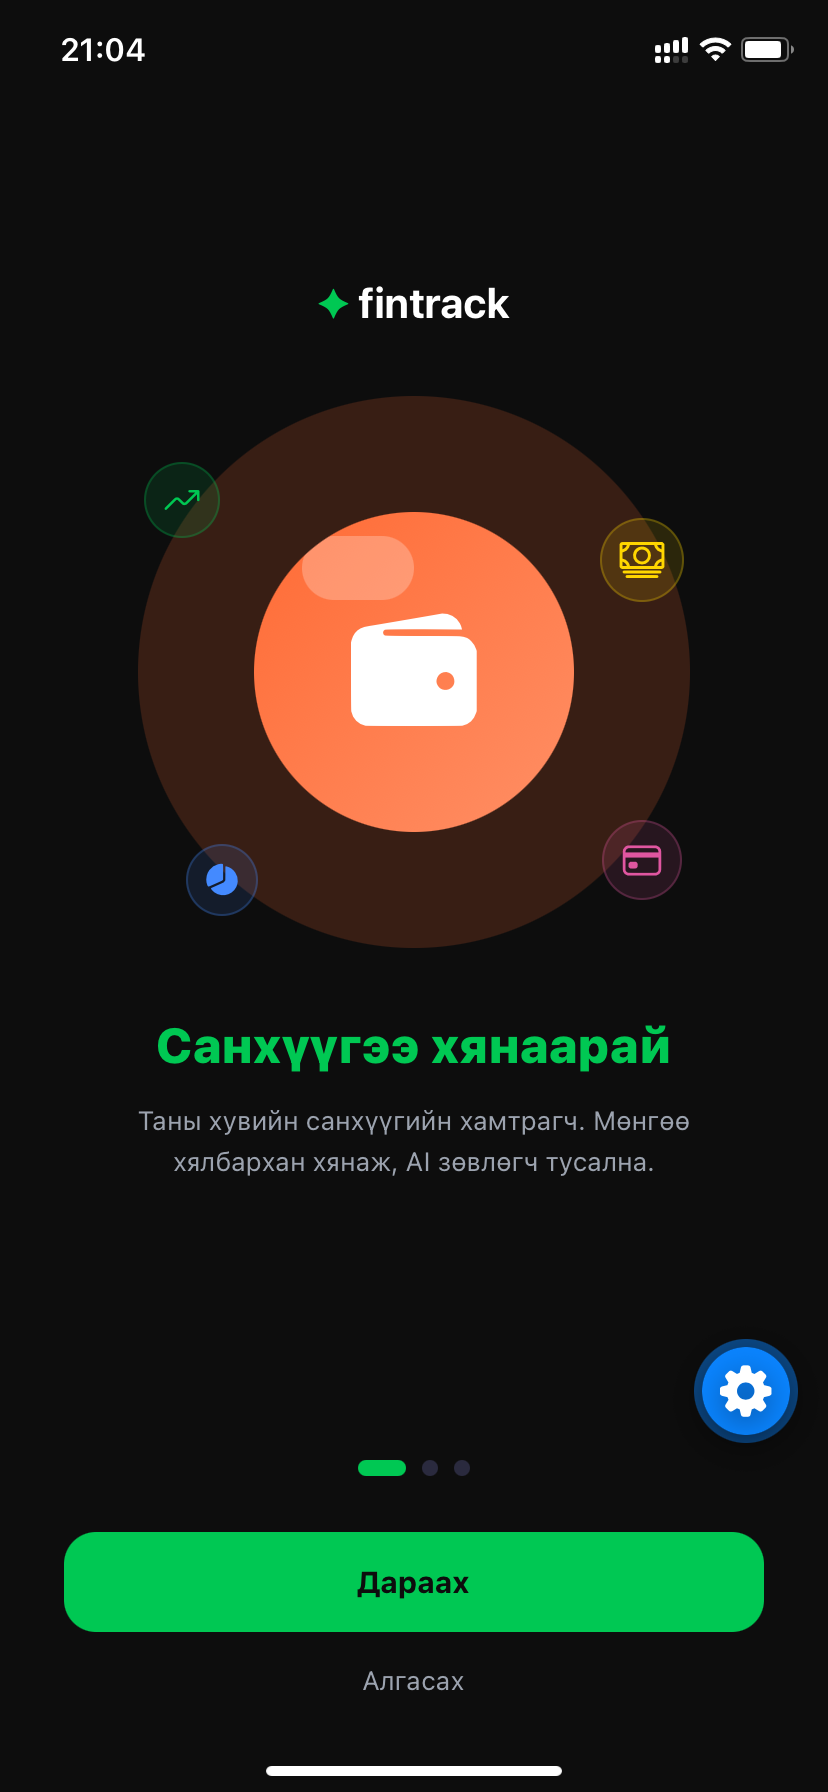
\includegraphics[width=\textwidth]{Figures/screen_onboarding_1.png}
    \caption{Санхүүгээ хяна}
    \label{fig:onboarding-1}
\end{subfigure}
\hfill
\begin{subfigure}[t]{0.24\textwidth}
    \centering
    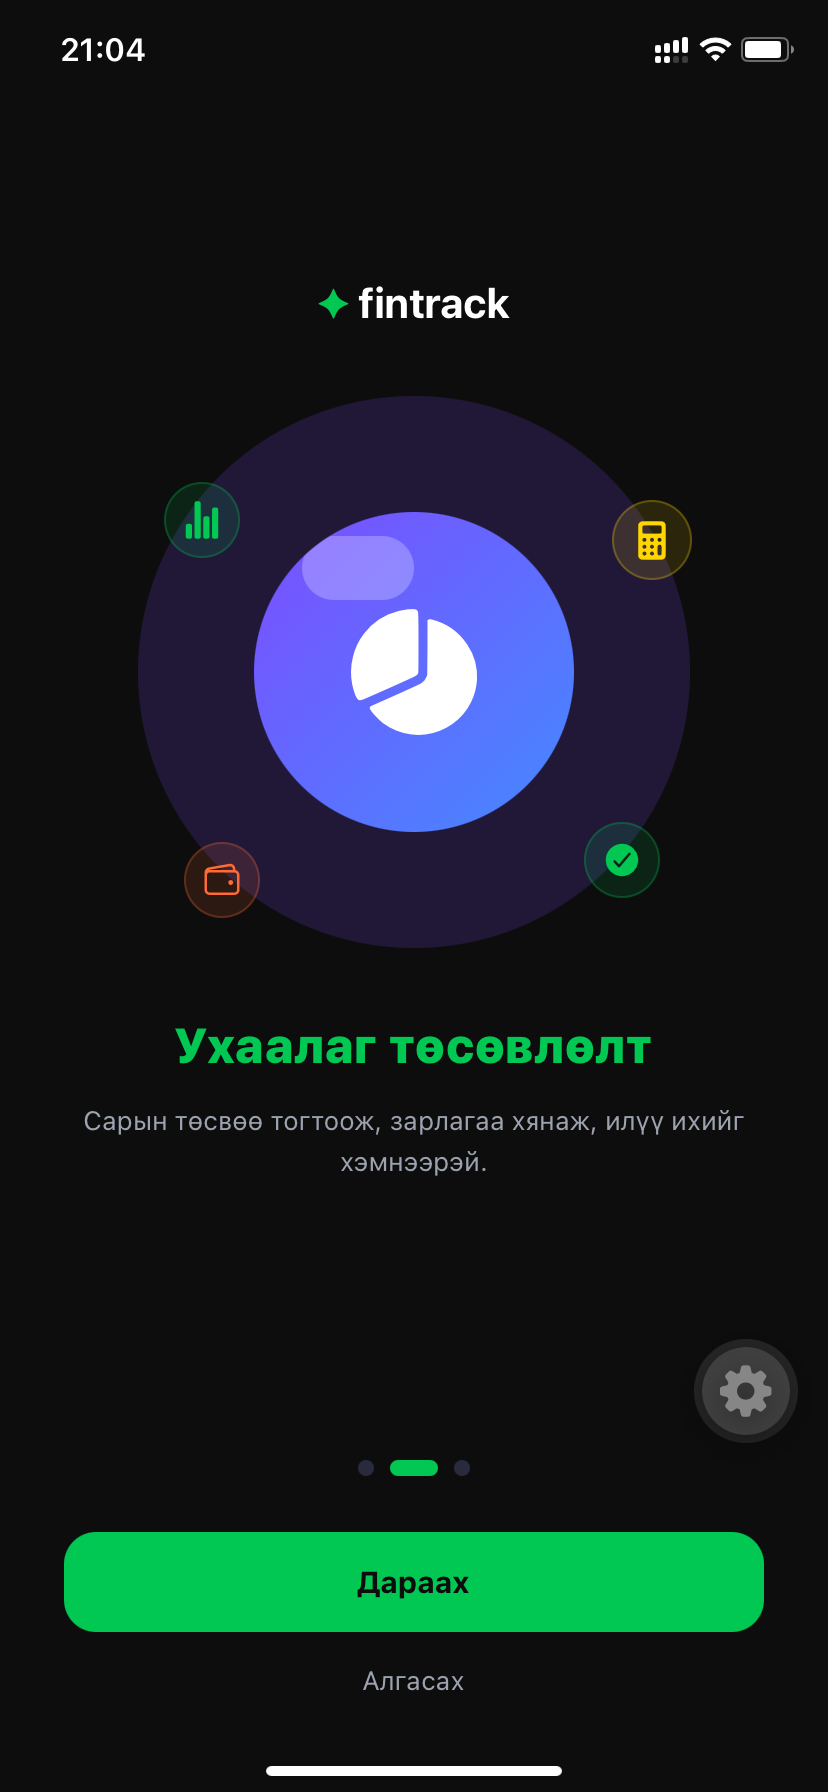
\includegraphics[width=\textwidth]{Figures/screen_onboarding_2.png}
    \caption{Ухаалаг төсөвлөлт}
    \label{fig:onboarding-2}
\end{subfigure}
\hfill
\begin{subfigure}[t]{0.24\textwidth}
    \centering
    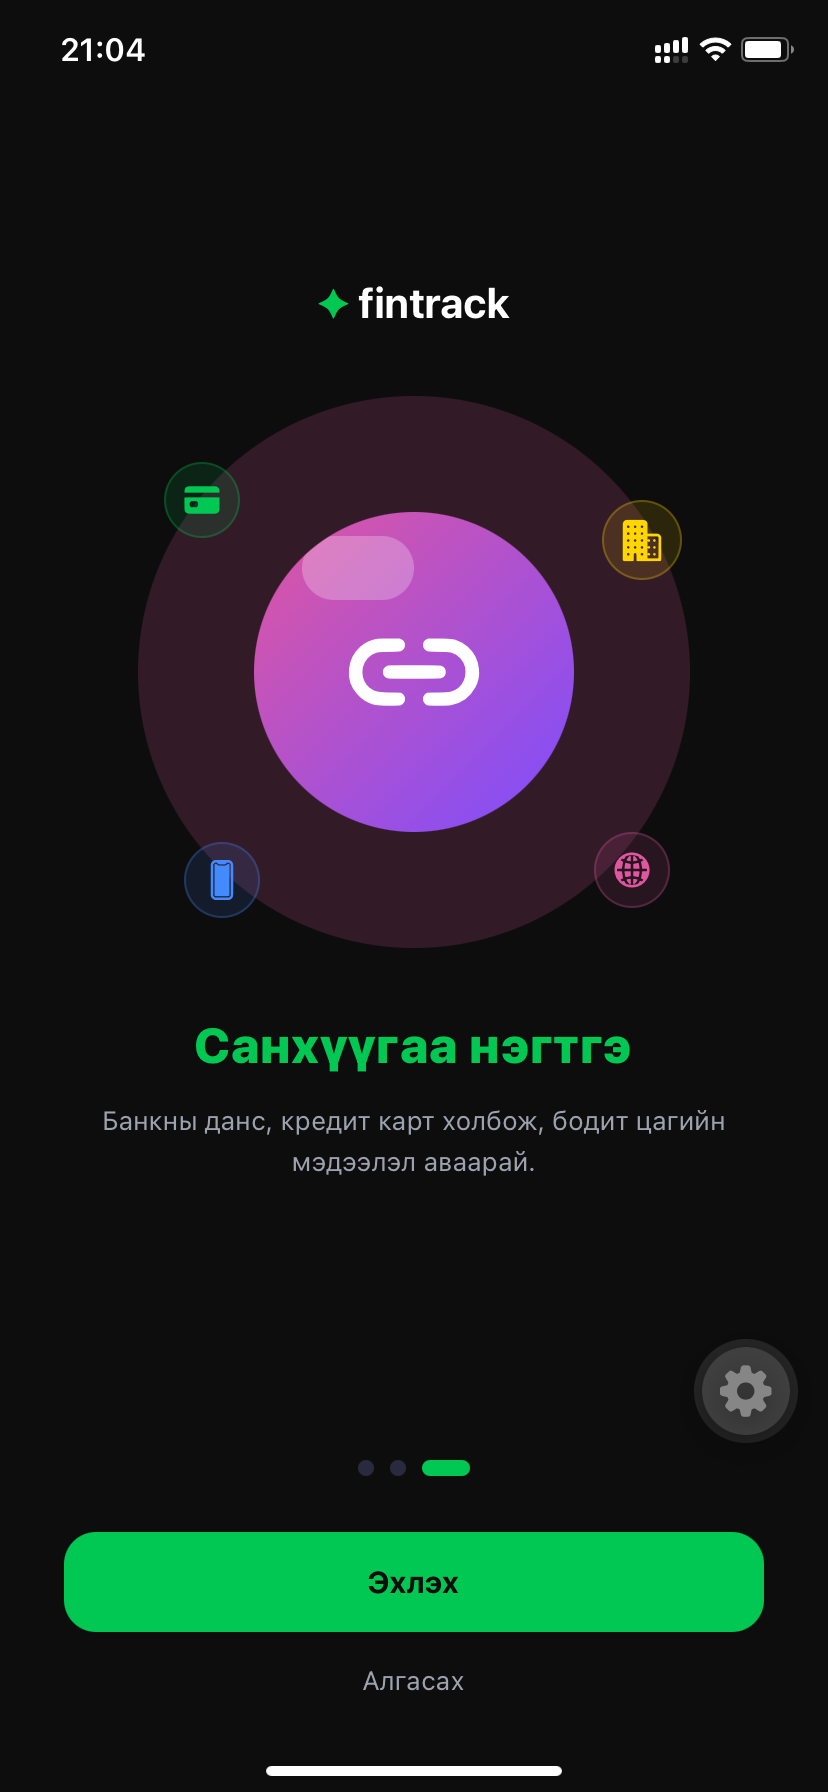
\includegraphics[width=\textwidth]{Figures/screen_onboarding_3.png}
    \caption{Санхүүгээ нэгтгэ}
    \label{fig:onboarding-3}
\end{subfigure}
\caption{Танилцах гурван үе шат}
\label{fig:onboarding}
\end{figure}

\textbf{Гол элементүүд:}
\begin{itemize}
    \item \textbf{Алхам бүрд том дугуй дүрс} (хэтэвч, диаграмм, холбоосын дүрс) гол санааг визуал хэлбэрээр илэрхийлнэ.
    \item \textbf{Гарчиг ба тайлбар} --- хэрэглэгчид программын зорилгыг товчоор тайлбарлана.
    \item \textbf{Доод хэсгийн явцын цэгүүд} --- хэрэглэгч одоогийн алхамаа хардаг.
    \item \textbf{"Дараах" ба "Алгасах" товчлуурууд} --- сонгож үргэлжлүүлэх боломж.
\end{itemize}

Танилцах хэсгийг дуусгаад хэрэглэгчид \textbf{бүртгэлийн дэлгэц} нээгдэнэ. Энд хэрэглэгч бүтэн нэр, имэйл, нууц үг, утасны дугаараа оруулж бүртгүүлнэ. Мөн Facebook, Google, Apple ID-аар нэвтрэх боломжтой.

\begin{figure}[H]
\centering
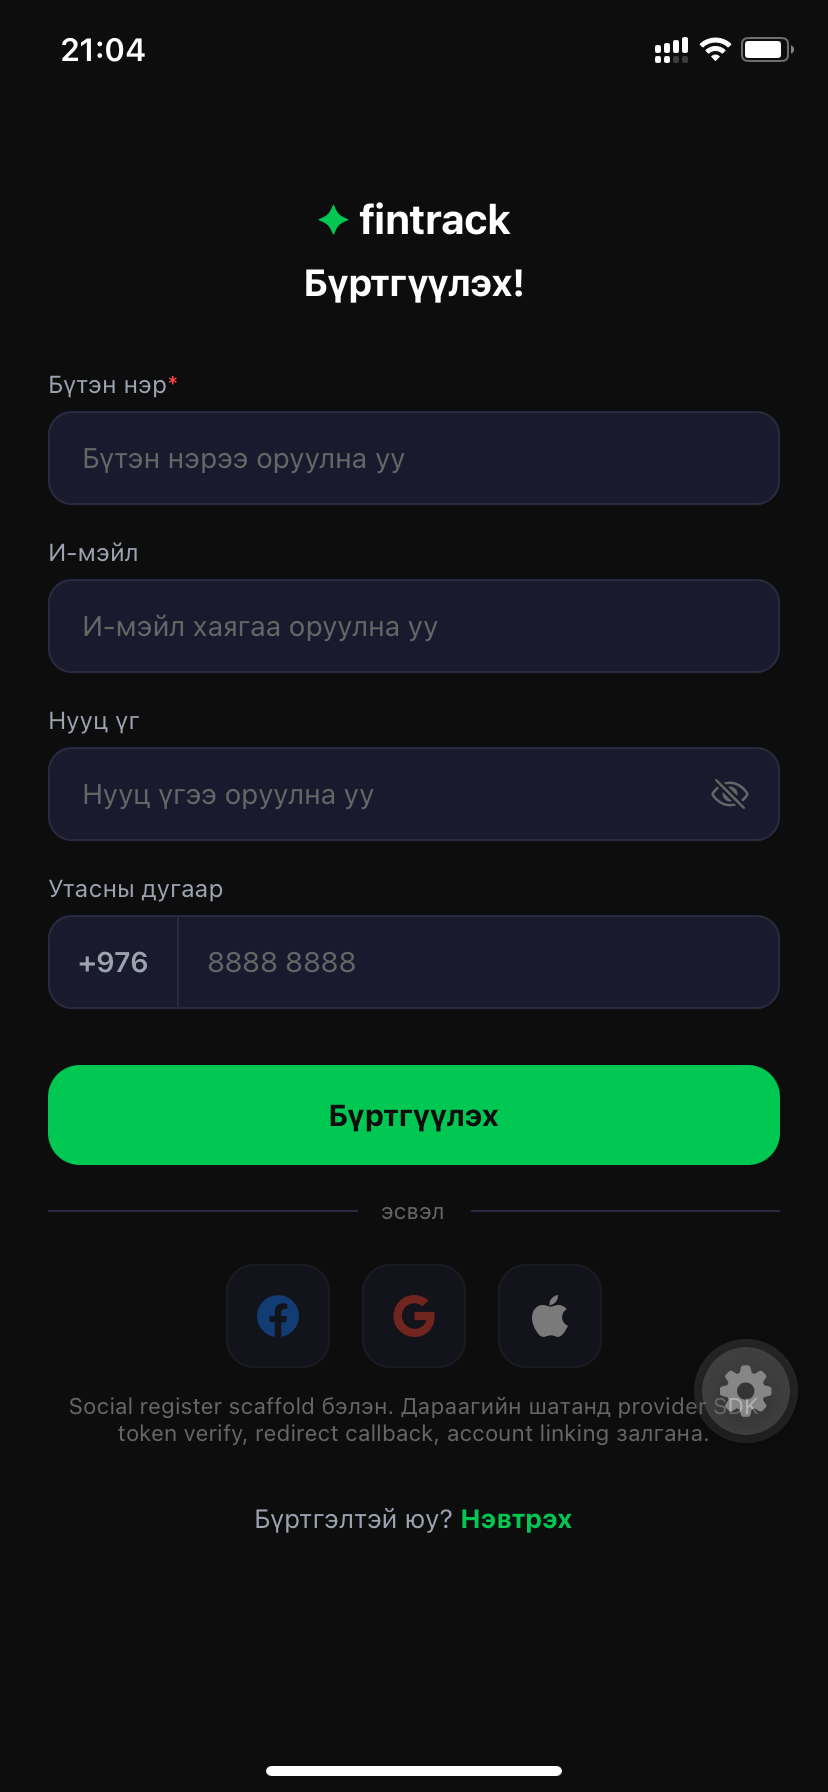
\includegraphics[width=0.36\textwidth]{Figures/screen_register.png}
\caption{Бүртгэлийн дэлгэц --- имэйл, нууц үг болон нийгмийн сүлжээний нэвтрэлтийн сонголтууд}
\label{fig:register}
\end{figure}

\textbf{Ар талын логик.} \texttt{POST /api/v1/auth/register} API цэг рүү \texttt{full\_name}, \texttt{email}, \texttt{password}, \texttt{phone} илгээгдэнэ. Сервер bcrypt cost=10-аар нууц үгийг хэшилж, JWT (HS256, 24 цаг) олгоно. Хэрэглэгч бүртгэгдэхэд автоматаар "Main Account" нэртэй анхдагч данс үүсгэдэг.

Хэрэглэгч нууц үгээ мартсан тохиолдолд \emph{"Нууц үгээ мартсан уу?"} холбоосоор дамжуулан \textbf{ForgotPassword} дэлгэц рүү шилжинэ. Тэнд имэйл хаягаа оруулахад \texttt{POST /api/v1/auth/forgot-password} API цэг рүү хүсэлт явж, бүртгэлтэй имэйл рүү нэг удаагийн сэргээх токен илгээгдэнэ.

\section{Нүүр дэлгэц}
Хэрэглэгч нэвтэрсний дараа хамгийн түрүүнд харагдах дэлгэц бол \textbf{нүүр} (Home) дэлгэц юм. Энэ дэлгэц нь хэрэглэгчийн санхүүгийн ерөнхий байдлыг нэг харахад ойлгуулах зорилготой.

\begin{figure}[H]
\centering
\begin{subfigure}[t]{0.28\textwidth}
    \centering
    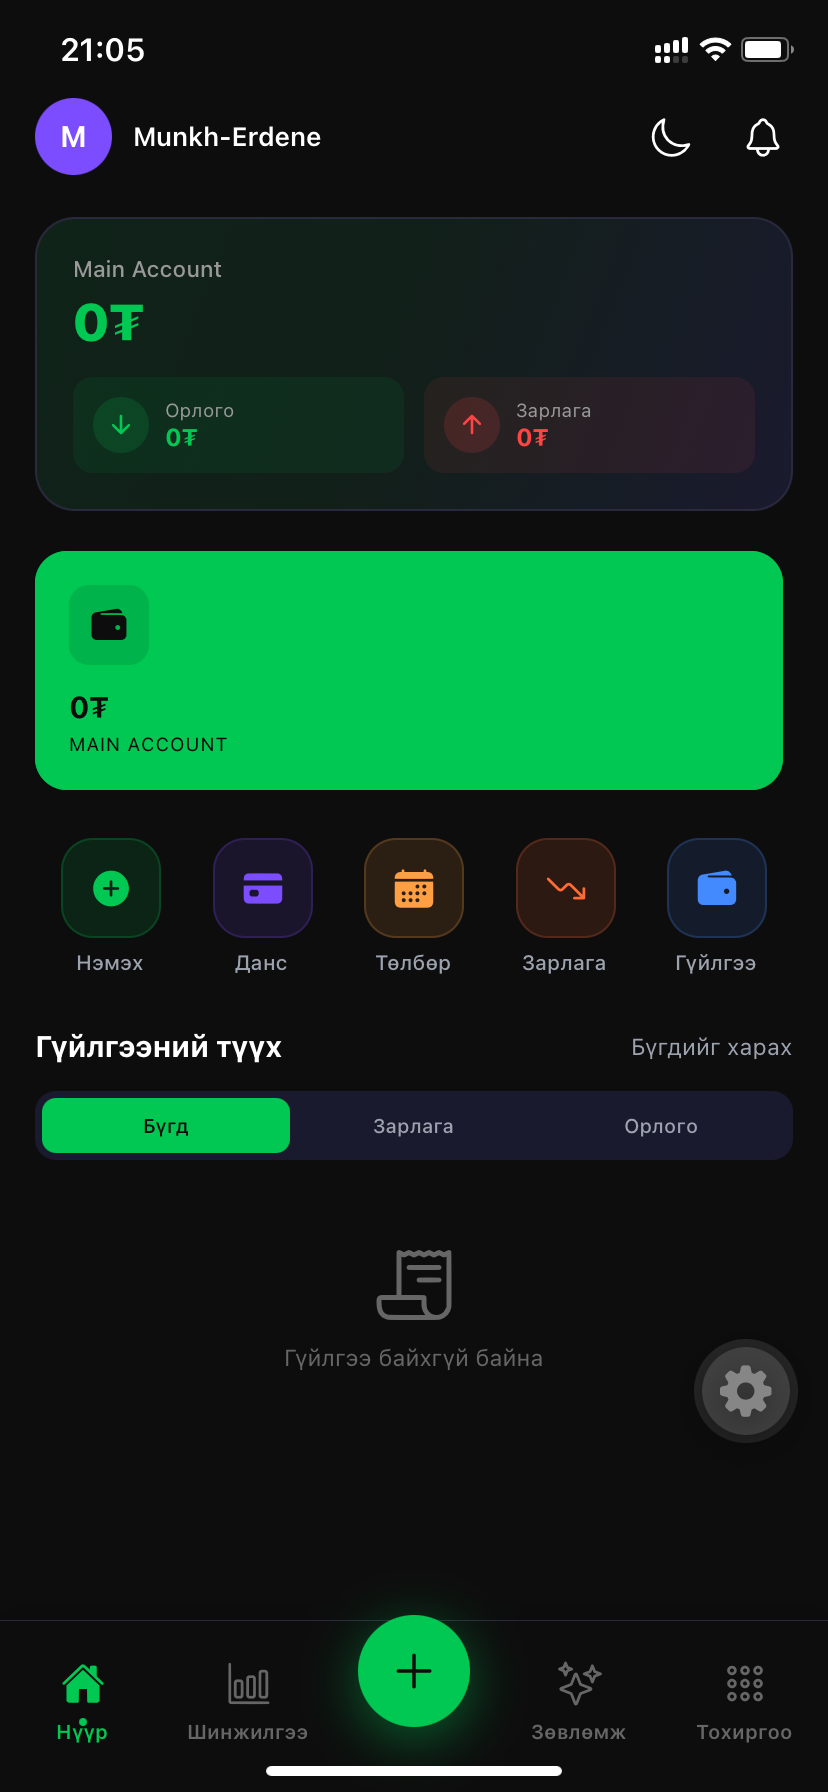
\includegraphics[width=\textwidth]{Figures/screen_home_initial.png}
    \caption{Анхны хоосон төлөв}
    \label{fig:home-initial}
\end{subfigure}
\hfill
\begin{subfigure}[t]{0.28\textwidth}
    \centering
    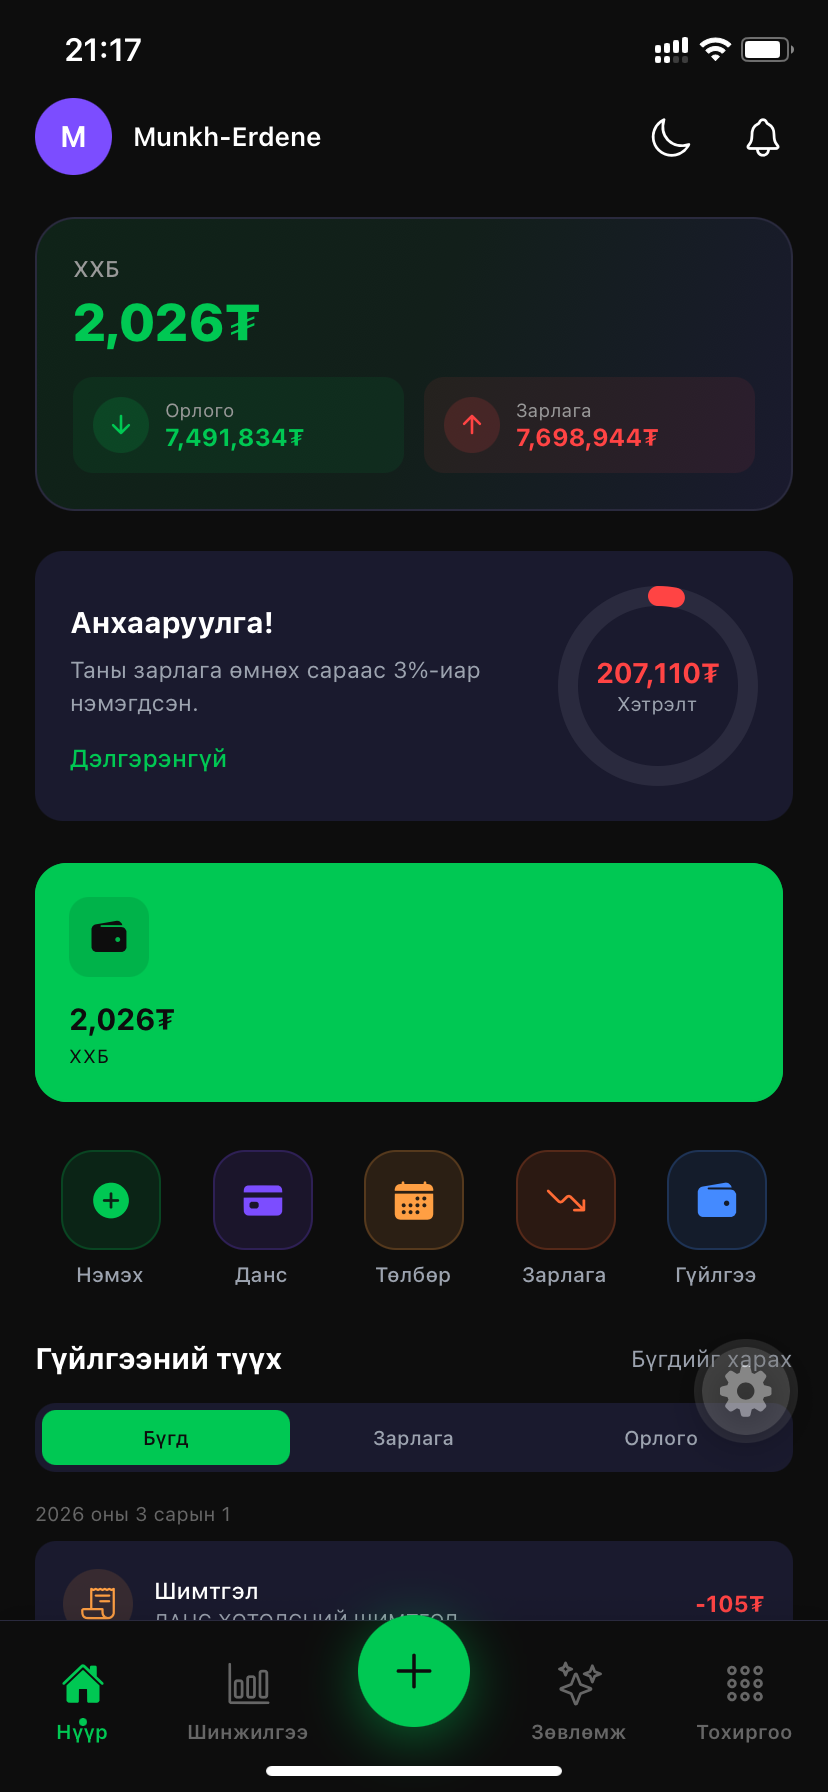
\includegraphics[width=\textwidth]{Figures/screen_home_xxb.png}
    \caption{ХХБ сонгогдсон төлөв}
    \label{fig:home-xxb}
\end{subfigure}
\hfill
\begin{subfigure}[t]{0.28\textwidth}
    \centering
    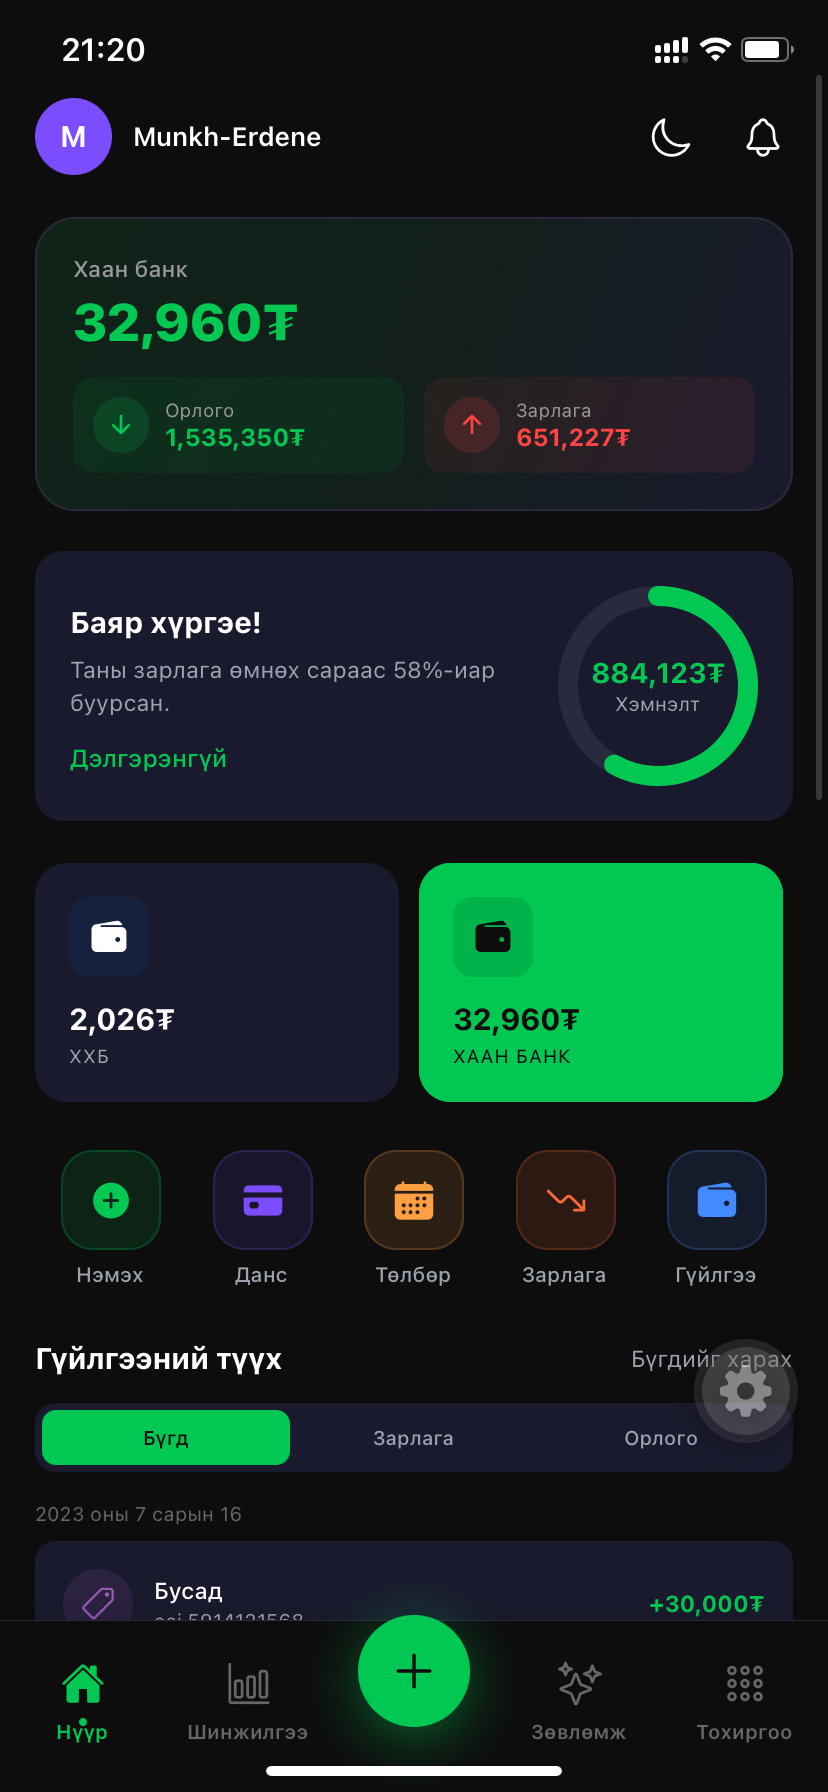
\includegraphics[width=\textwidth]{Figures/screen_home_khan.png}
    \caption{Хаан банк сонгогдсон төлөв}
    \label{fig:home-khan}
\end{subfigure}
\caption{Нүүр дэлгэц --- идэвхтэй дансаар хувирах байдал}
\label{fig:home-screens}
\end{figure}

\textbf{Гол элементүүд:}
\begin{itemize}
    \item \textbf{Толгой мөр.} Зүүн талд хэрэглэгчийн аватар, нэр (Munkh-Erdene); баруун талд харанхуй/гэрэлтэй горим солих сарны тэмдэг ба мэдэгдлийн хонх.
    \item \textbf{Идэвхтэй дансны карт.} Сонгосон банкны нэр, одоогийн үлдэгдэл (Хаан банк дээр 32{,}960 төг, ХХБ дээр 2{,}026 төг), сарын орлого, зарлагын богино нэгтгэл.
    \item \textbf{Хэмнэлт буюу хэтрэлтийн дугуй прогресс.} Өмнөх сартай харьцуулсан үр дүнг (Хаан банк дээр 58\% буурсан хэмнэлт, ХХБ дээр 3\% нэмэгдсэн хэтрэлт) тойрог хэлбэрээр харуулна. Хэмнэлт ногоон, хэтрэлт улаан өнгөтэй.
    \item \textbf{Дансны хайрцгууд.} Хэрэглэгчийн бүх банкны данс зэрэгцэн харагдана. Дарвал тухайн данс идэвхтэй болж бүх тоо, диаграмм шинэчлэгдэнэ.
    \item \textbf{Хурдан үйлдлүүд.} \emph{Нэмэх}, \emph{Данс}, \emph{Төлбөр}, \emph{Зарлага}, \emph{Гүйлгээ} гэсэн 5 шууд товчлуур.
    \item \textbf{Гүйлгээний түүх.} \emph{Бүгд}, \emph{Зарлага}, \emph{Орлого} гэсэн 3 шүүлтүүртэй сүүлийн гүйлгээний жагсаалт.
    \item \textbf{Доод хэсгийн цэс.} Нүүр, Шинжилгээ, +, Зөвлөмж (AI), Тохиргоо гэсэн 5 үндсэн дэлгэц.
\end{itemize}

\textbf{Ар талын логик.} Нүүр дэлгэц нээгдэхэд клиент талаас \texttt{GET /api/v1/dashboard} API цэг рүү хүсэлт явна. Сервер нь \texttt{DashboardResponse} объектыг буцаадаг бөгөөд дотор нь нийт үлдэгдэл, сарын орлого, зарлага, хэмнэлтийн хувь, бүх данс, сүүлийн 10 гүйлгээ багтсан байна. Уг хариултыг \texttt{src/services/api.ts} модуль хүлээн авч HomeScreen-д харуулна.

\section{Дансны удирдлага}
Хэрэглэгч олон банкны дансаа нэгэн зэрэг хадгалж, удирдах боломжтой. Анх бүртгэгдэх үед "Main Account" нэртэй анхдагч данс автоматаар үүсдэг бөгөөд хэрэглэгч өөр данс нэмж, устгаж, засаж болно.

\begin{figure}[H]
\centering
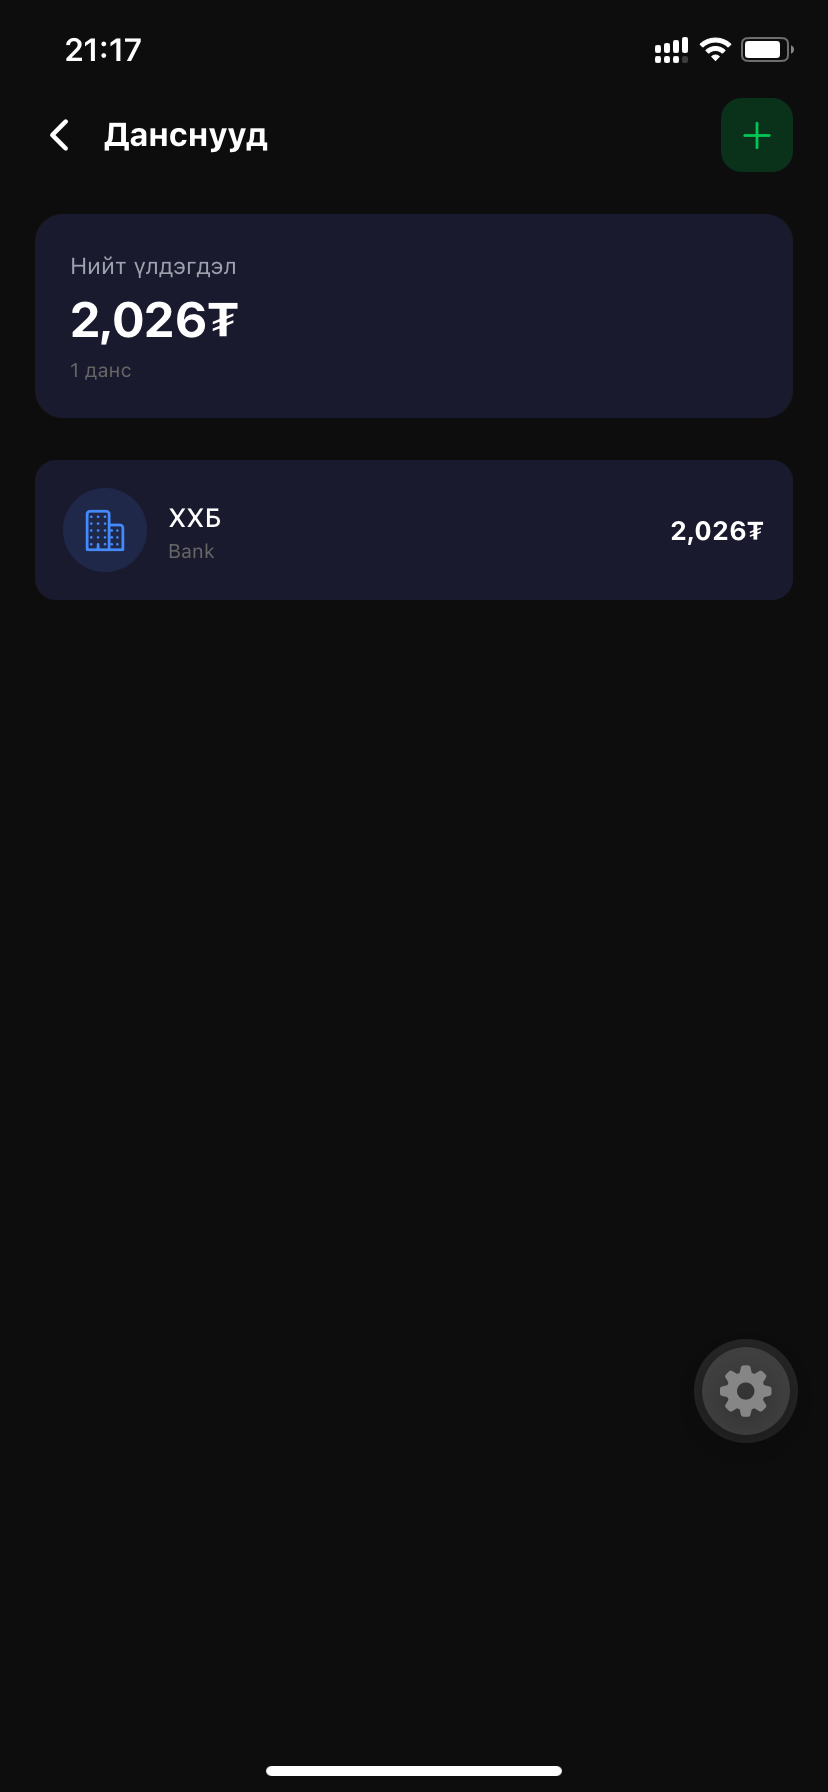
\includegraphics[width=0.36\textwidth]{Figures/screen_accounts.png}
\caption{Дансны жагсаалт --- нийт үлдэгдэл ба идэвхтэй данс}
\label{fig:accounts}
\end{figure}

\textbf{Гол элементүүд:}
\begin{itemize}
    \item \textbf{Нийт үлдэгдэл.} Бүх дансны нийлбэрийг том үсгээр харуулна. Доор нь хэдэн данстай байгааг тоогоор бичсэн.
    \item \textbf{Дансны карт.} Дансны нэр (ХХБ), төрөл (Bank), үлдэгдэл (2{,}026 төг).
    \item \textbf{Шинэ данс нэмэх товчлуур.} Баруун дээд буланд байрлах ногоон \texttt{+} товчлуур.
\end{itemize}

\textbf{Ар талын логик.} Бүх дансыг \texttt{GET /api/v1/accounts}-аас унших ба \texttt{POST}, \texttt{PUT}, \texttt{DELETE} HTTP аргуудаар CRUD хийгдэнэ. Гүйлгээний мэдээлэл өөрчлөгдөх бүрд GORM-ийн hook ажиллаж тухайн дансны үлдэгдэл автоматаар шинэчлэгддэг.

\section{Гүйлгээ нэмэх}
Шинэ орлого, зарлагын гүйлгээг \texttt{+} товчлуур дарж нэмнэ. Дэлгэц нь хүснэгт хэлбэрээр зохион байгуулагдсан бөгөөд хэрэглэгч хамгийн цөөн товшилтоор гүйлгээгээ бүртгэж чаддаг. Зарлага сонгосон үед улаан, орлого сонгосон үед ногоон өнгөөр будагдан, хэрэглэгчийн хэсгийн өнгө өөрчлөгддөг.

\begin{figure}[H]
\centering
\begin{subfigure}[t]{0.36\textwidth}
    \centering
    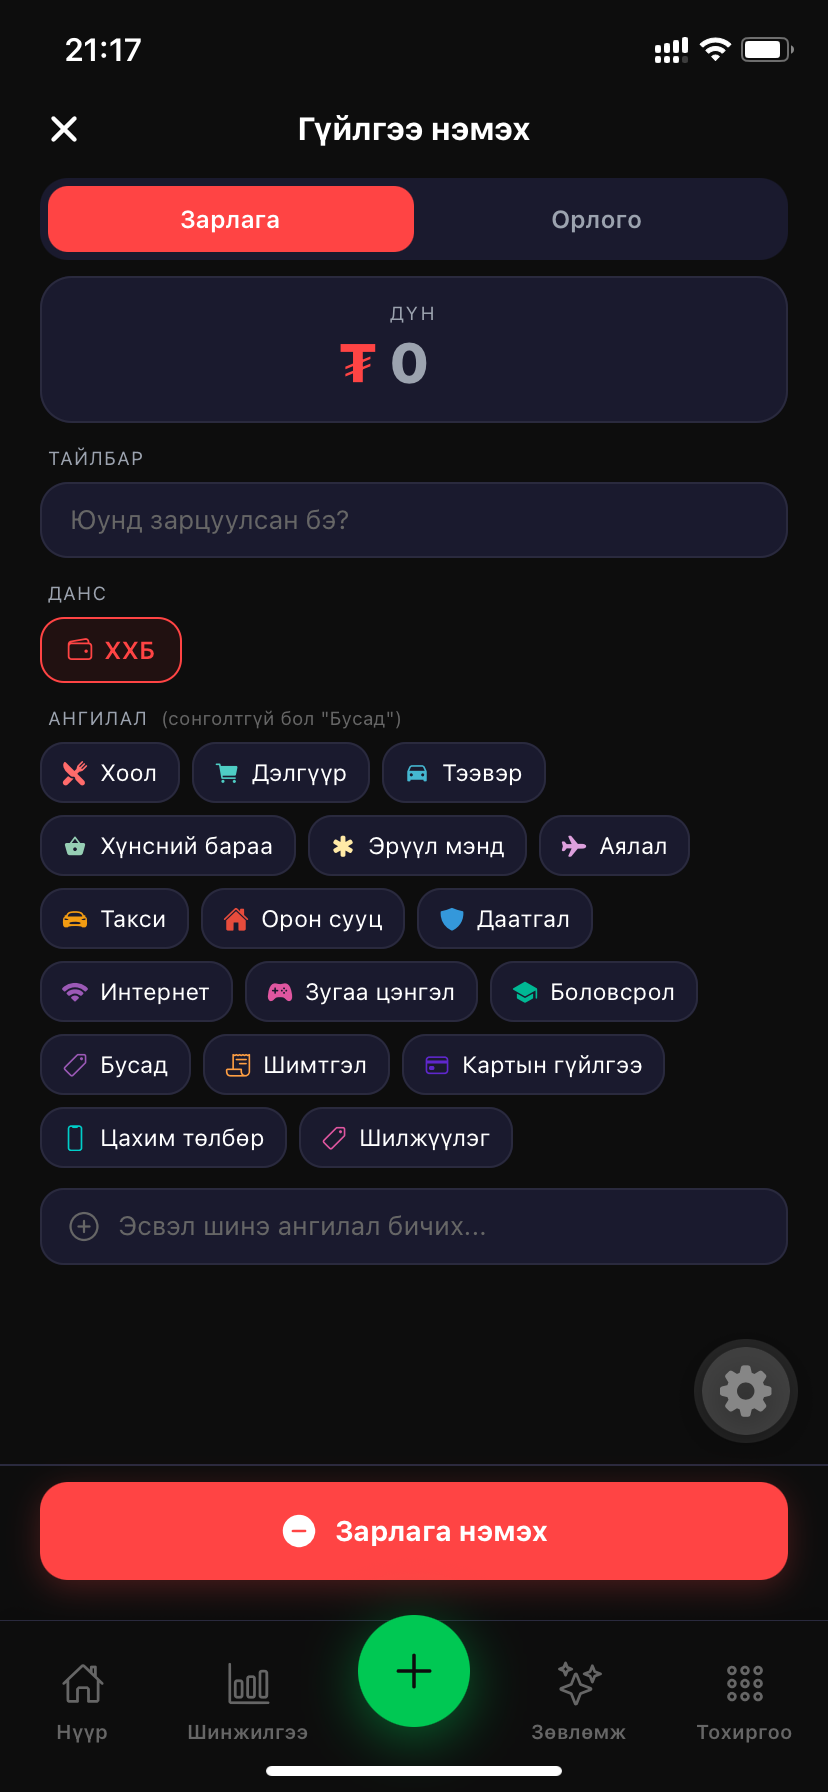
\includegraphics[width=\textwidth]{Figures/screen_addtx_expense.png}
    \caption{Зарлага нэмэх (улаан)}
    \label{fig:addtx-expense}
\end{subfigure}
\hfill
\begin{subfigure}[t]{0.36\textwidth}
    \centering
    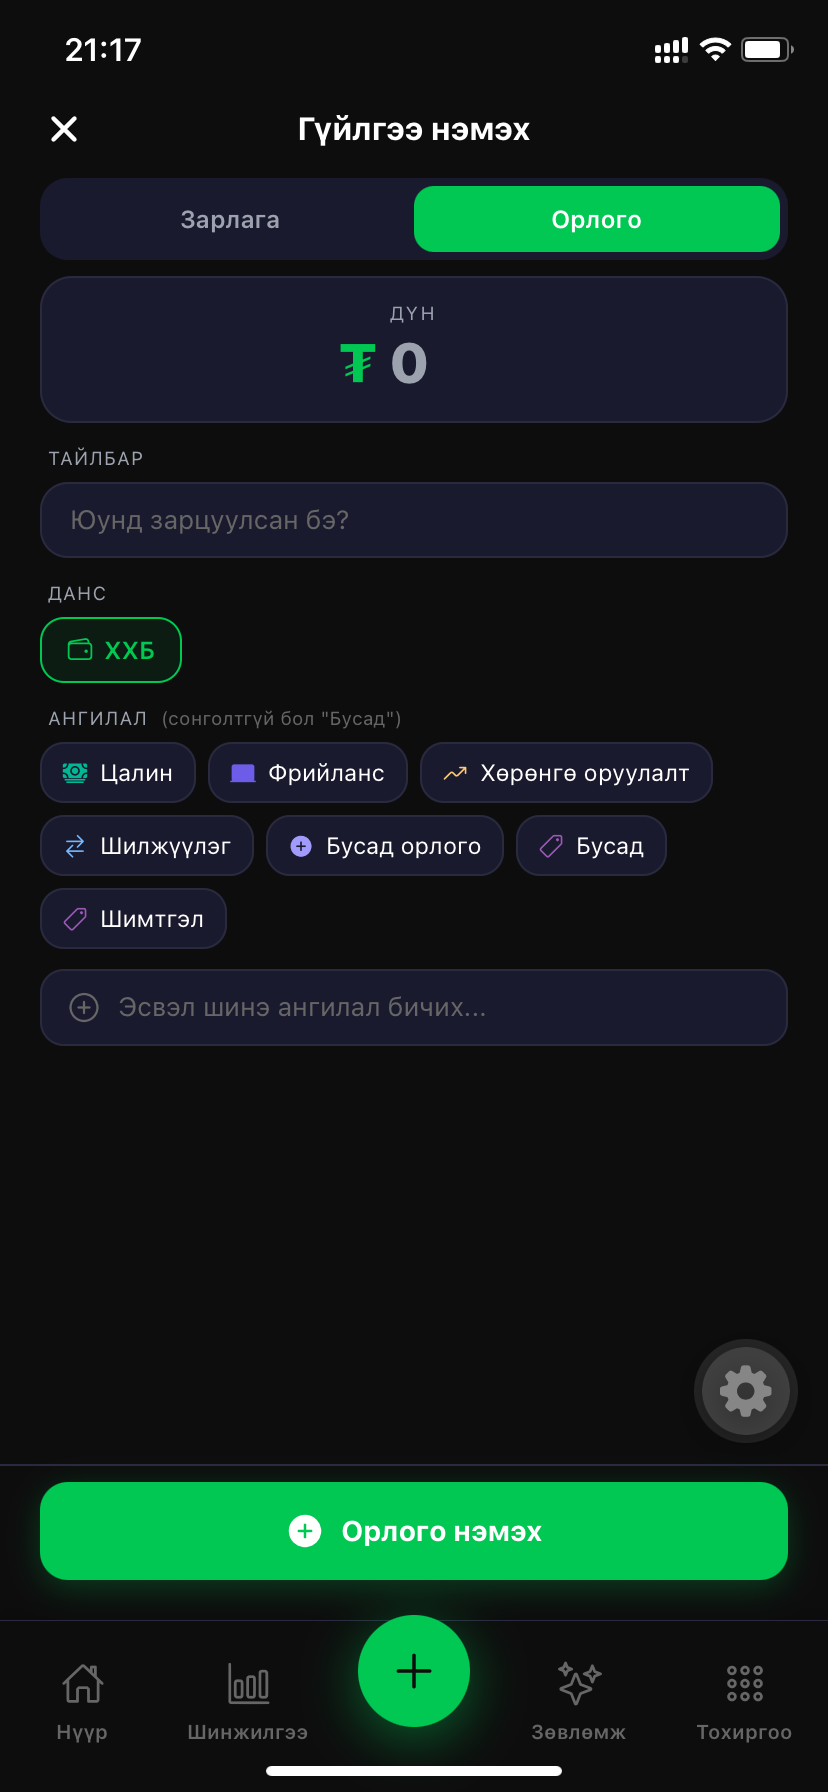
\includegraphics[width=\textwidth]{Figures/screen_addtx_income.png}
    \caption{Орлого нэмэх (ногоон)}
    \label{fig:addtx-income}
\end{subfigure}
\caption{Гүйлгээ нэмэх дэлгэц --- зарлага ба орлогын горим}
\label{fig:addtx}
\end{figure}

\textbf{Гол элементүүд:}
\begin{itemize}
    \item \textbf{Төрөл сонголт.} \emph{Зарлага} ба \emph{Орлого} гэсэн хоёр таб. Сонгосон таб нь өнгөтэй (зарлага улаан, орлого ногоон) болж тодорно.
    \item \textbf{Дүн оруулах талбар.} Том төгрөгийн тэмдэгтэй тоон оролт. Хэрэглэгч гар утасны цифр гараас оруулна.
    \item \textbf{Тайлбар.} "Юунд зарцуулсан бэ?" гэсэн байрлуулах тексттэй оролт. Сүүлд нь AI ангилахад туслах нэмэлт мэдээлэл болно.
    \item \textbf{Данс сонгох.} Хэрэглэгчийн бүх банкны жагсаалт. Анхдагчаар идэвхтэй дансыг сонгоно.
    \item \textbf{Ангилал.} Зарлагын хувьд 17 ангилал (Хоол, Дэлгүүр, Тээвэр, Хүнсний бараа, Эрүүл мэнд, Аялал, Такси, Орон сууц, Даатгал, Интернэт, Зугаа цэнгэл, Боловсрол, Бусад, Шимтгэл, Картын гүйлгээ, Цахим төлбөр, Шилжүүлэг), орлогын хувьд 7 ангилал (Цалин, Фриланс, Хөрөнгө оруулалт, Шилжүүлэг, Бусад орлого, Бусад, Шимтгэл). Ангилал тус бүр өөрийн дүрс, өнгөтэй харагдана.
    \item \textbf{Шинэ ангилал бичих.} Үндсэн жагсаалтад байхгүй бол хэрэглэгч өөрөө шинэ ангилал нэмж бичих боломжтой.
    \item \textbf{Үндсэн товчлуур.} Дэлгэцийн доод хэсэгт байрлах "Зарлага нэмэх" буюу "Орлого нэмэх" том товчлуур.
\end{itemize}

\textbf{Ар талын логик.} \texttt{POST /api/v1/transactions} руу \texttt{CreateTransactionRequest} (account\_id, category\_id, amount, type, description, date) илгээнэ. Серверт оролтын баталгаажуулалт хийгдэн, GORM-аар Transaction бичлэг үүсэж, тухайн дансны үлдэгдэл нэмэгдэх буюу буурахаар шинэчлэгдэнэ. Үйлдлийг \texttt{ActivityLog} хүснэгтэд нэгэн зэрэг бүртгэнэ.

\section{Гүйлгээний түүх ба ангиллын задаргаа}
Нүүр дэлгэц дээрх "Бүгдийг харах" товч эсвэл хурдан үйлдлүүдийн "Зарлага", "Гүйлгээ" товчлуурууд нь дэлгэрэнгүй гүйлгээний түүх ба ангиллын задаргааны дэлгэцэд хүргэнэ.

\begin{figure}[H]
\centering
\begin{subfigure}[t]{0.28\textwidth}
    \centering
    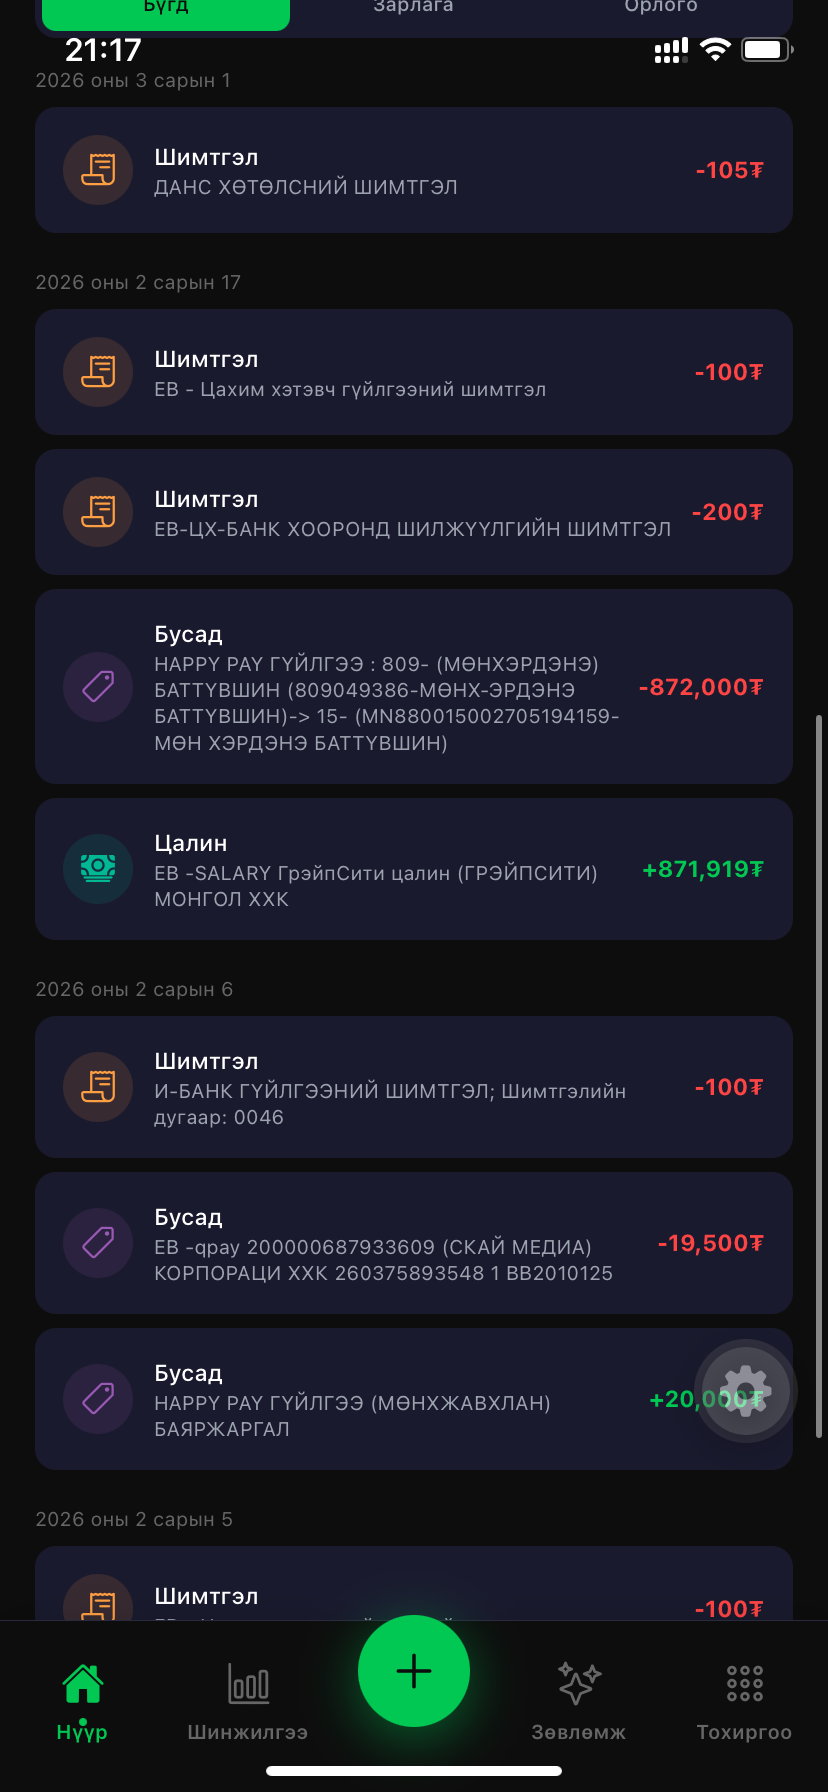
\includegraphics[width=\textwidth]{Figures/screen_history.png}
    \caption{Гүйлгээний түүх}
    \label{fig:history}
\end{subfigure}
\hfill
\begin{subfigure}[t]{0.28\textwidth}
    \centering
    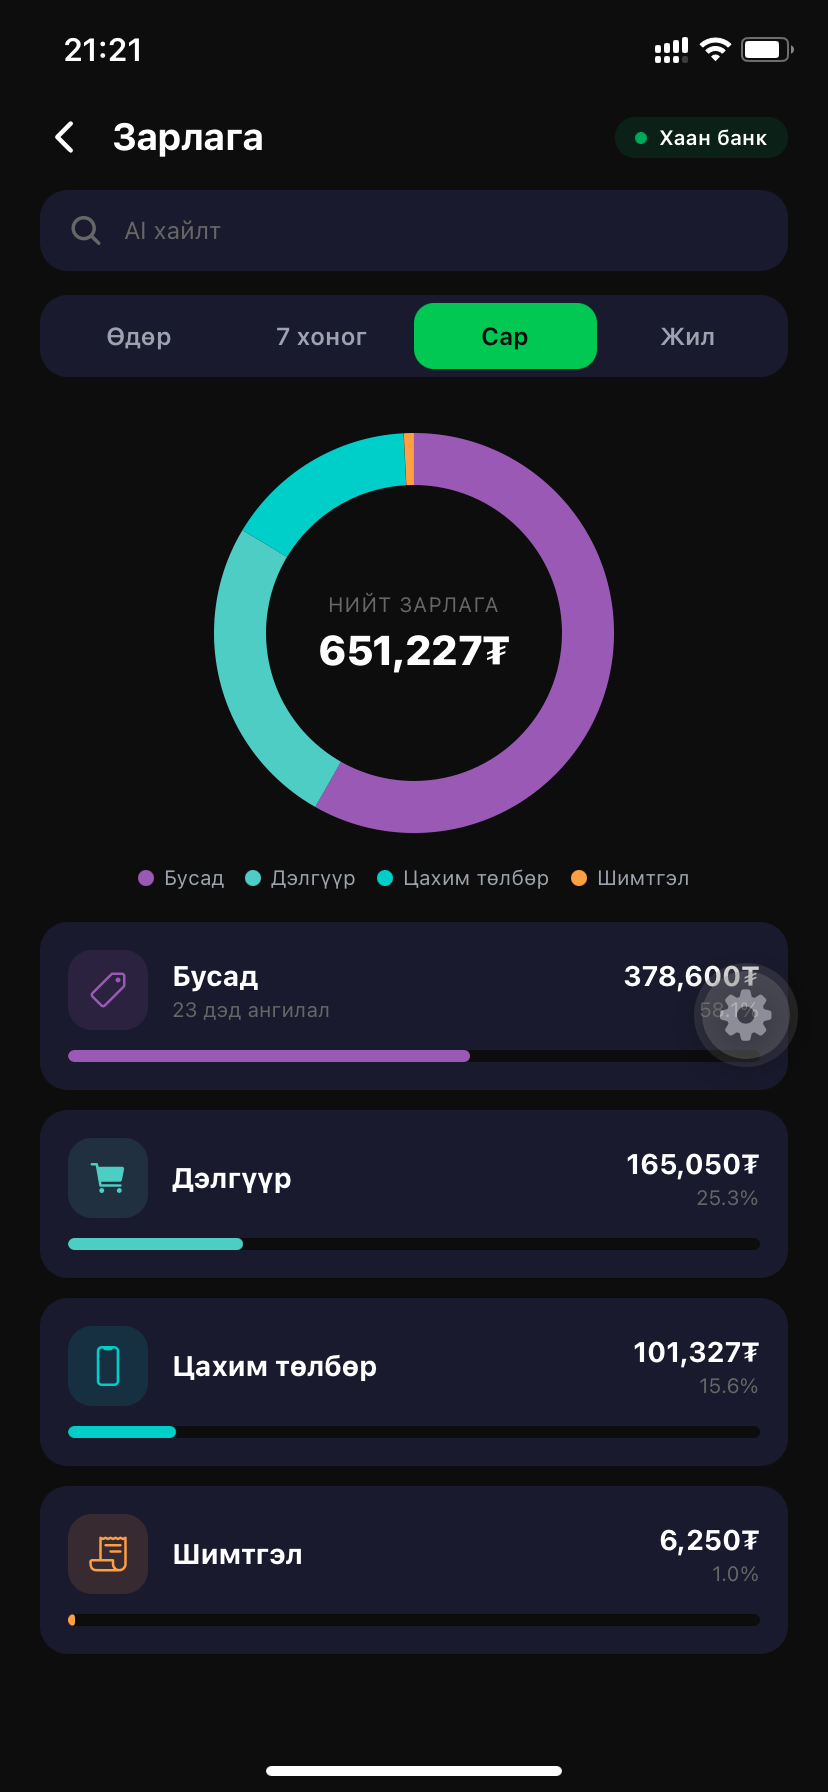
\includegraphics[width=\textwidth]{Figures/screen_expense_pie_khan.png}
    \caption{Хаан банк зарлагын pie chart}
    \label{fig:expense-pie-khan}
\end{subfigure}
\hfill
\begin{subfigure}[t]{0.28\textwidth}
    \centering
    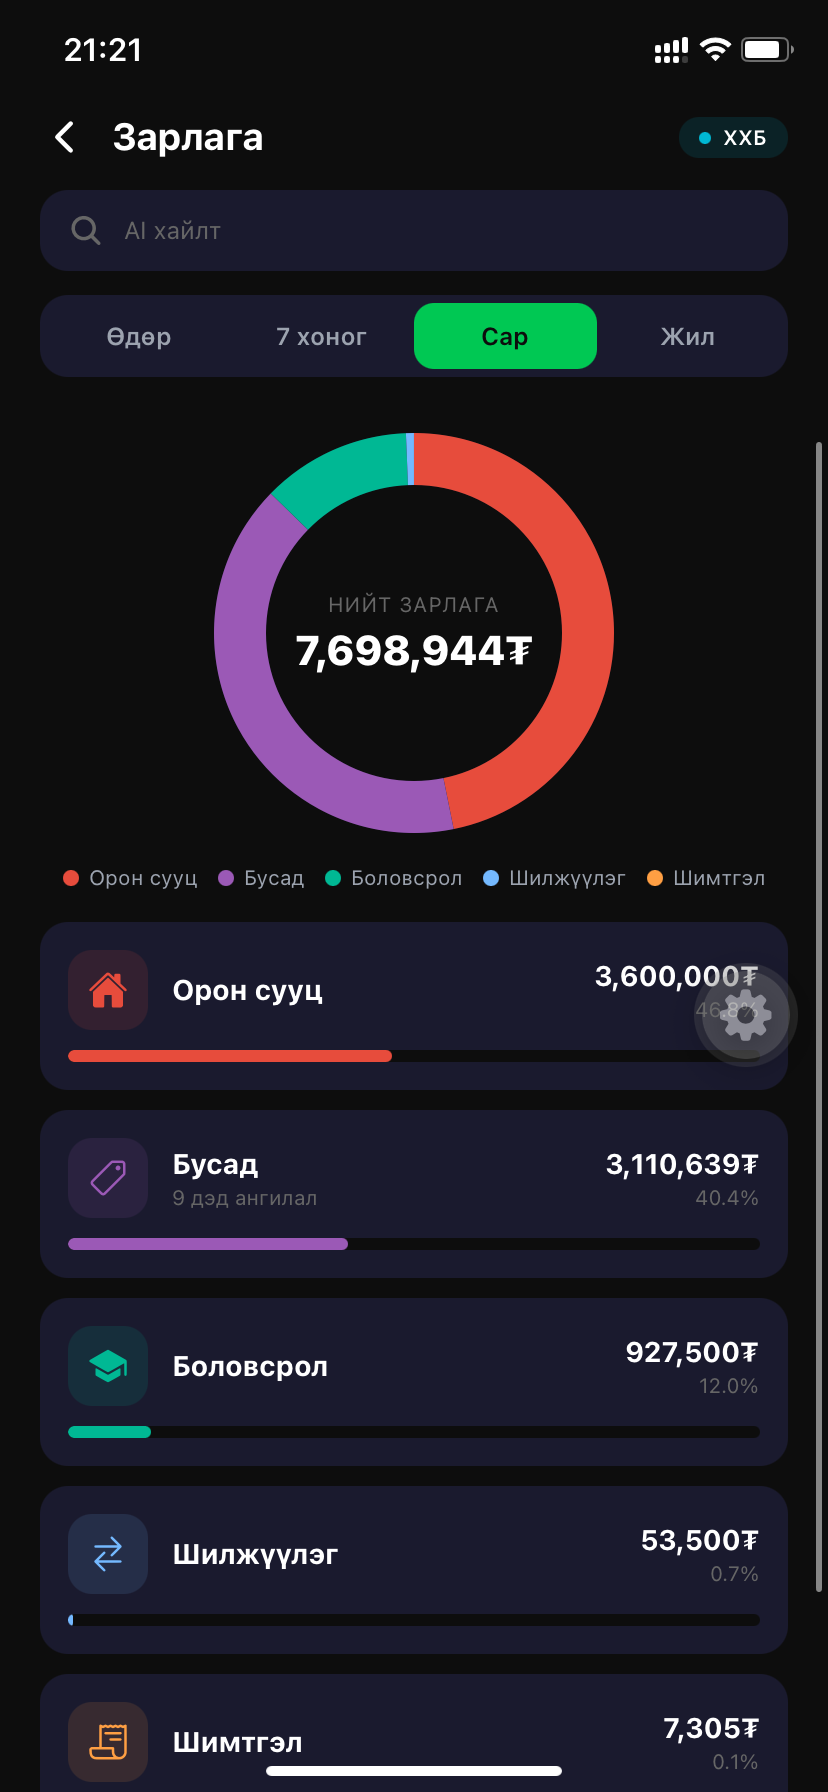
\includegraphics[width=\textwidth]{Figures/screen_expense_pie_xxb.png}
    \caption{ХХБ зарлагын pie chart}
    \label{fig:expense-pie-xxb}
\end{subfigure}
\caption{Гүйлгээний түүх ба ангиллын донат график}
\label{fig:history-pie}
\end{figure}

\textbf{Гол элементүүд:}
\begin{itemize}
    \item \textbf{Гүйлгээний түүх.} Огноогоор бүлэглэгдсэн гүйлгээний жагсаалт. Гүйлгээ бүр ангиллын дүрс, тайлбар, дүн (ногоон \texttt{+} нь орлого, улаан \texttt{-} нь зарлага)-тай харагдана.
    \item \textbf{AI хайлт.} Дээд хэсэгт байрлах хайлтын талбар нь чөлөөт хэлбэрийн асуултаар гүйлгээ хайх боломжийг олгоно (жишээ нь "сүүлийн 7 хоногийн хүнсний зардал").
    \item \textbf{Хугацааны шүүлтүүр.} \emph{Өдөр}, \emph{7 хоног}, \emph{Сар}, \emph{Жил} гэсэн 4 сонголт.
    \item \textbf{Донат график.} Зарлагын ангиллын задаргааг өнгөн ялгаатай дугуй график хэлбэрээр. Дунд хэсэгт нийт зарлагыг харуулна (Хаан банк дээр 651{,}227 төг, ХХБ дээр 7{,}698{,}944 төг).
    \item \textbf{Ангиллын жагсаалт.} Хамгийн их зарлагатай ангиллууд тоо, мөнгөн дүн, хувийн жинтэйгээр харагдана. Тус бүрийн явцын зурвас нь хувийг дүрслэн харуулна.
\end{itemize}

\textbf{Ар талын логик.} \texttt{GET /api/v1/transactions} API цэг нь огноо, ангилал, дансаар шүүгдсэн жагсаалт буцаана. \texttt{GET /api/v1/expenses/breakdown?period=monthly} нь ангилал тус бүрийн нийт зарлагыг нэгтгэн буцаадаг. AI хайлт нь \texttt{POST /api/v1/transactions/search} API цэг рүү ердийн хэлээр бичсэн асуулга илгээж, LLM-ийг ашиглан SQL руу хөрвүүлэн хайлт хийнэ.

\section{Шинжилгээ дэлгэц --- статистик горим}
Шинжилгээ дэлгэц нь хоёр горимтой: \textbf{Статистик} (тоон үзүүлэлт + багана график) болон \textbf{Диаграмм} (гөлгөр муруй). Хэрэглэгч өдөр, 7 хоног, сар, жил гэсэн хугацааны шүүлтүүр сонгож харах боломжтой.

\begin{figure}[H]
\centering
\begin{subfigure}[t]{0.36\textwidth}
    \centering
    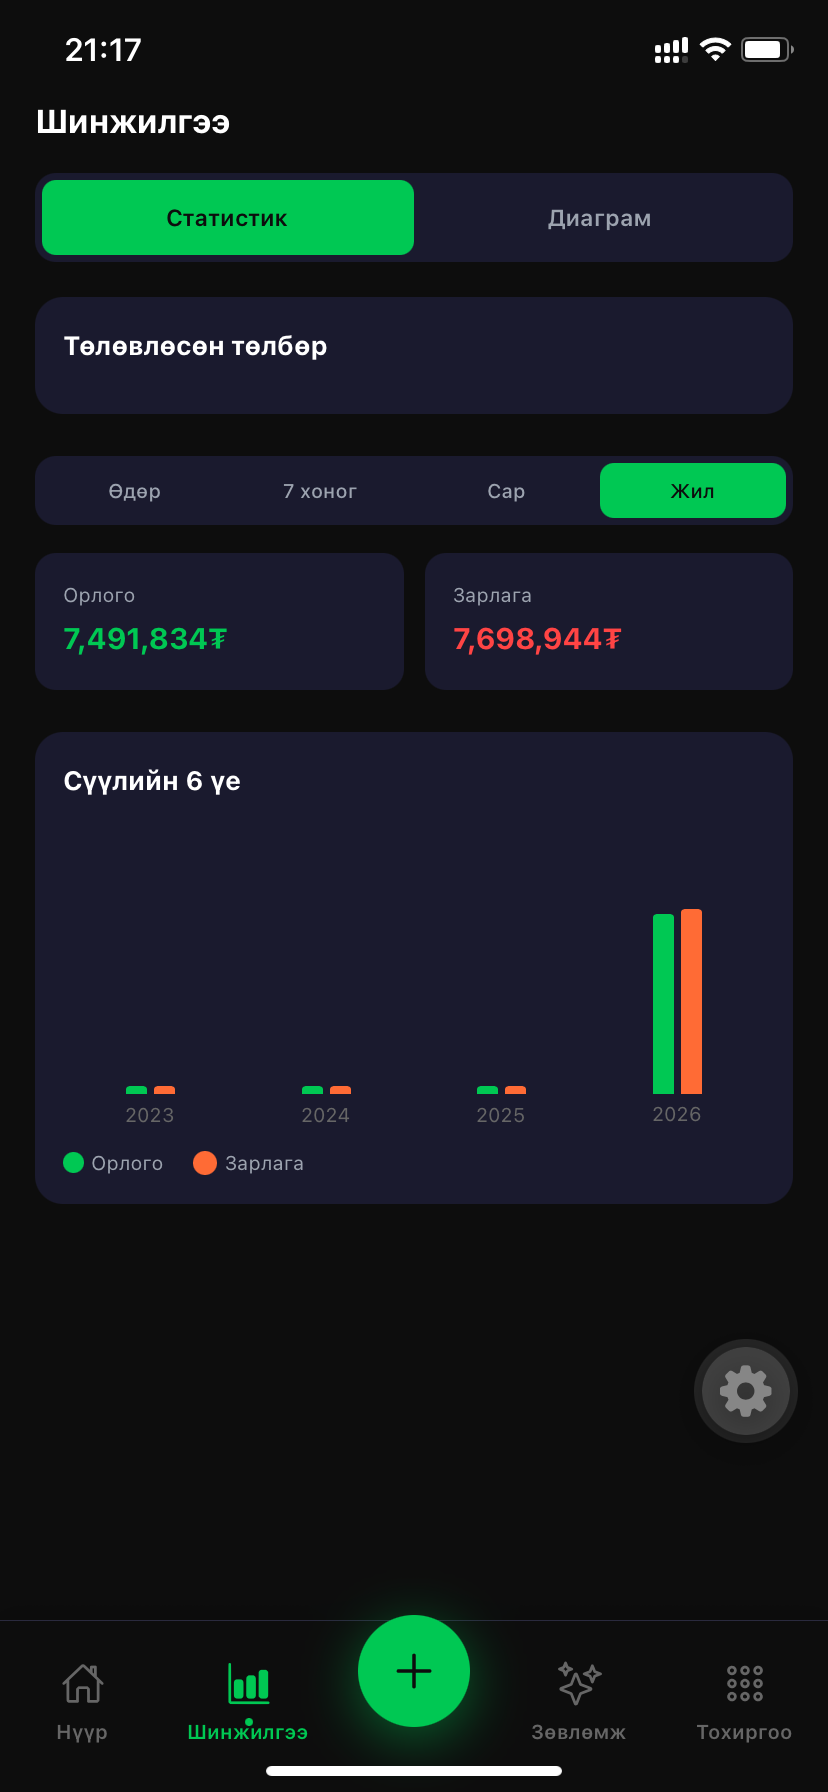
\includegraphics[width=\textwidth]{Figures/screen_stats_year_all.png}
    \caption{Жил --- бүх данс нэгтгэн}
    \label{fig:stats-year-all}
\end{subfigure}
\hfill
\begin{subfigure}[t]{0.36\textwidth}
    \centering
    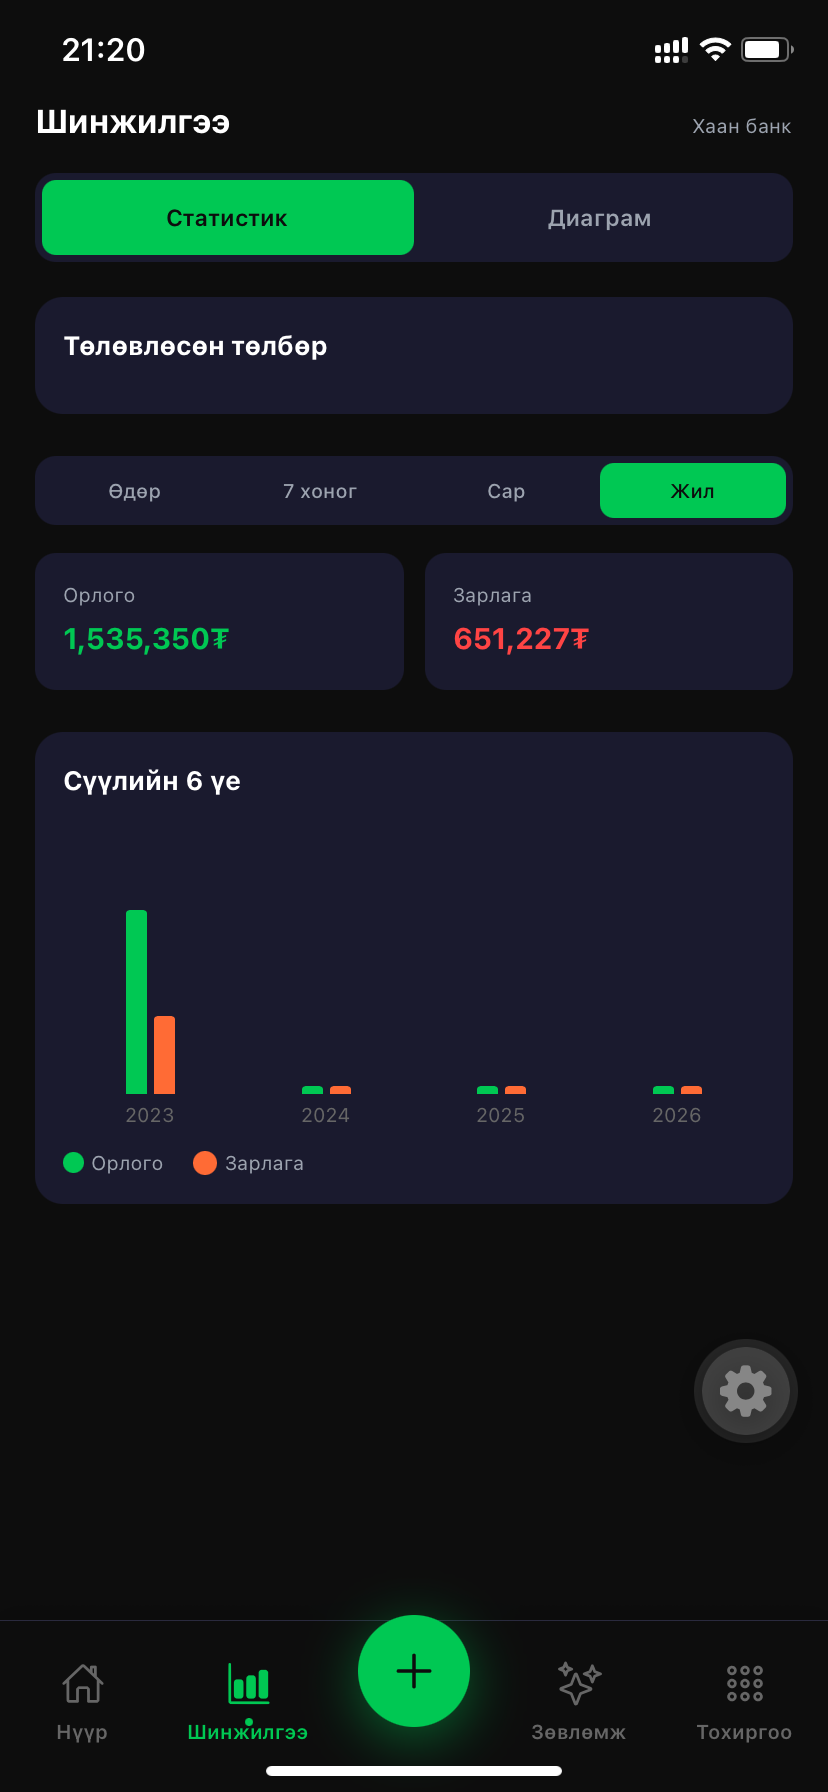
\includegraphics[width=\textwidth]{Figures/screen_stats_year_khan.png}
    \caption{Жил --- Хаан банк}
    \label{fig:stats-year-khan}
\end{subfigure}
\caption{Статистик горим --- орлого, зарлагын тоон нэгтгэл ба 6 жилийн харьцуулалт}
\label{fig:stats-screens}
\end{figure}

\textbf{Гол элементүүд:}
\begin{itemize}
    \item \textbf{Дээд таб.} \emph{Статистик} ба \emph{Диаграмм} гэсэн хоёр горимыг солих.
    \item \textbf{Хугацааны шүүлтүүр.} \emph{Өдөр}, \emph{7 хоног}, \emph{Сар}, \emph{Жил} гэсэн 4 сонголтын шүүлтүүр. Сонгогдсон сонголт ногоон тодорсон төлөвөөр харагдана.
    \item \textbf{Идэвхтэй данс.} Баруун дээд буланд тухайн харагдаж байгаа дансны нэр (Хаан банк).
    \item \textbf{Орлого, Зарлагын карт.} Тухайн хугацаан дахь нийлбэрийг ногоон, улаан өнгөөр харуулна (7{,}491{,}834 төг орлого, 7{,}698{,}944 төг зарлага).
    \item \textbf{Сүүлийн 6 үе.} Багана графикаар орлого, зарлагыг харьцуулна. 2023-2025 онуудад бага хэмжээтэй, 2026 онд хамгийн өндөр гүйлгээтэй байгаа нь харагдана.
    \item \textbf{Төлөвлөсөн төлбөрийн нэгтгэл.} Дээд хэсэгт давтагдах төлбөрүүдийн нийт мөнгөн дүнг харуулдаг.
\end{itemize}

\textbf{Ар талын логик.} \texttt{GET /api/v1/statistics?period=yearly} зэрэг асуулгын параметр нь сервер тал дээрх \texttt{dashboard.go:GetStatistics} боловсруулагчийг дуудна. Сервер тухайн хугацаанд хамаарах гүйлгээг GORM-аар нэгтгэн 6 үеийн өгөгдлийг буцаана. Хэрэглэгч тал нь \texttt{react-native-chart-kit} санг ашиглан багана графикийг хөрвүүлэн харуулдаг.

\section{Шинжилгээ дэлгэц --- диаграмм горим}
Диаграмм горим нь орлого, зарлагын чиг хандлагыг \emph{гөлгөр муруй} хэлбэрээр харуулна. Энэ нь нэгэн харахад чиг хандлагыг ойлгоход тохиромжтой.

\begin{figure}[H]
\centering
\begin{subfigure}[t]{0.36\textwidth}
    \centering
    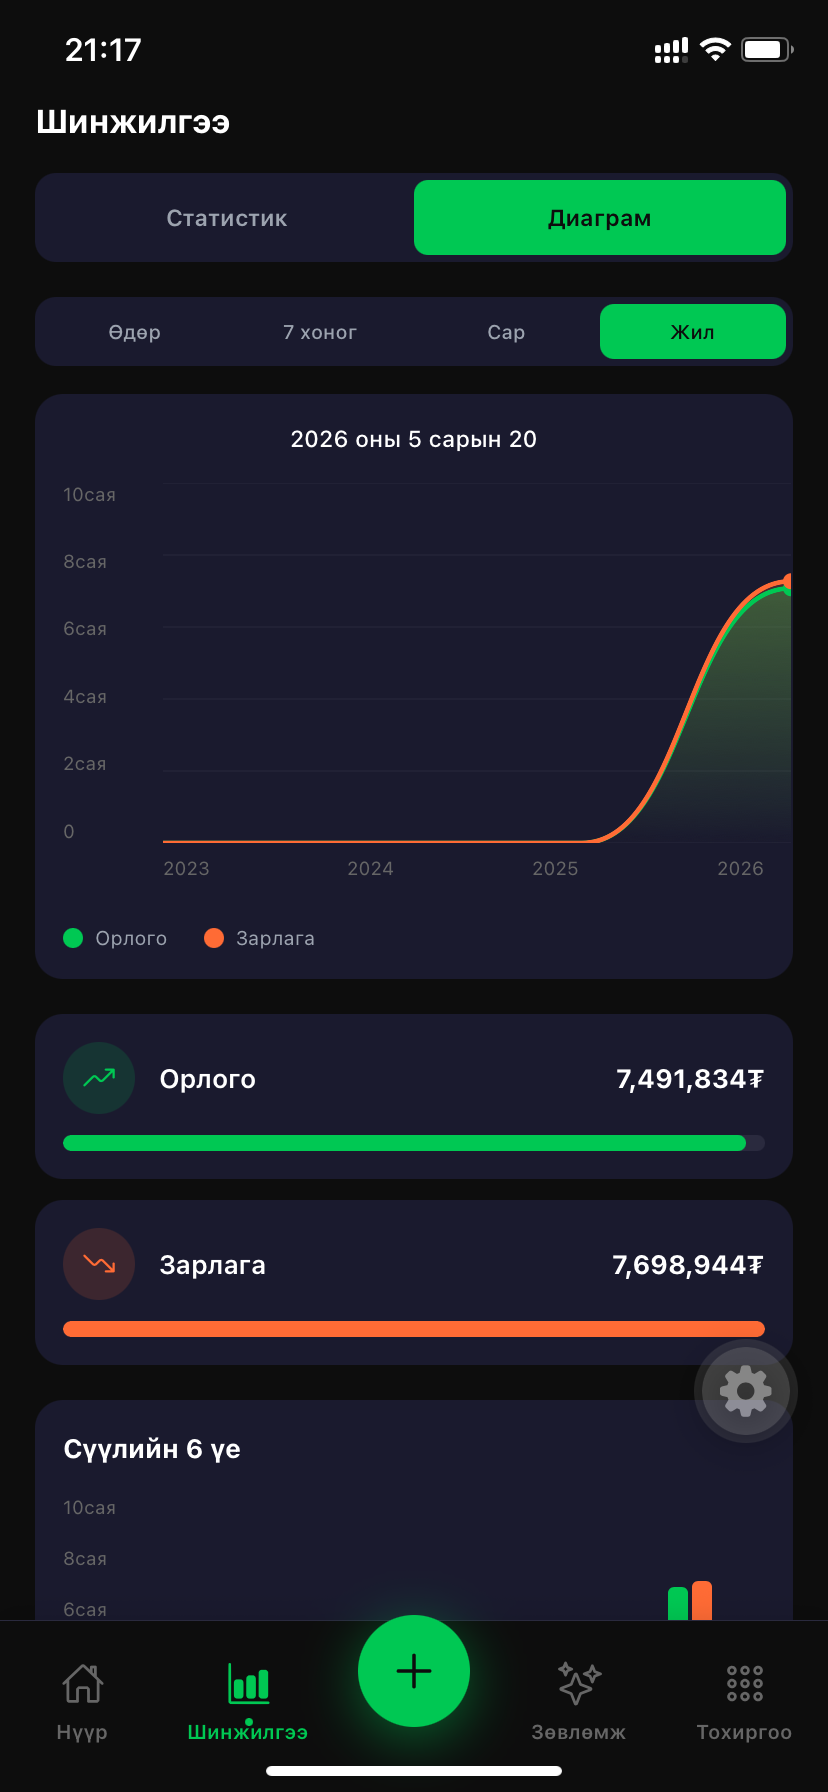
\includegraphics[width=\textwidth]{Figures/screen_chart_year_all.png}
    \caption{Жил --- бүх данс (2023--2026)}
    \label{fig:chart-year-all}
\end{subfigure}
\hfill
\begin{subfigure}[t]{0.36\textwidth}
    \centering
    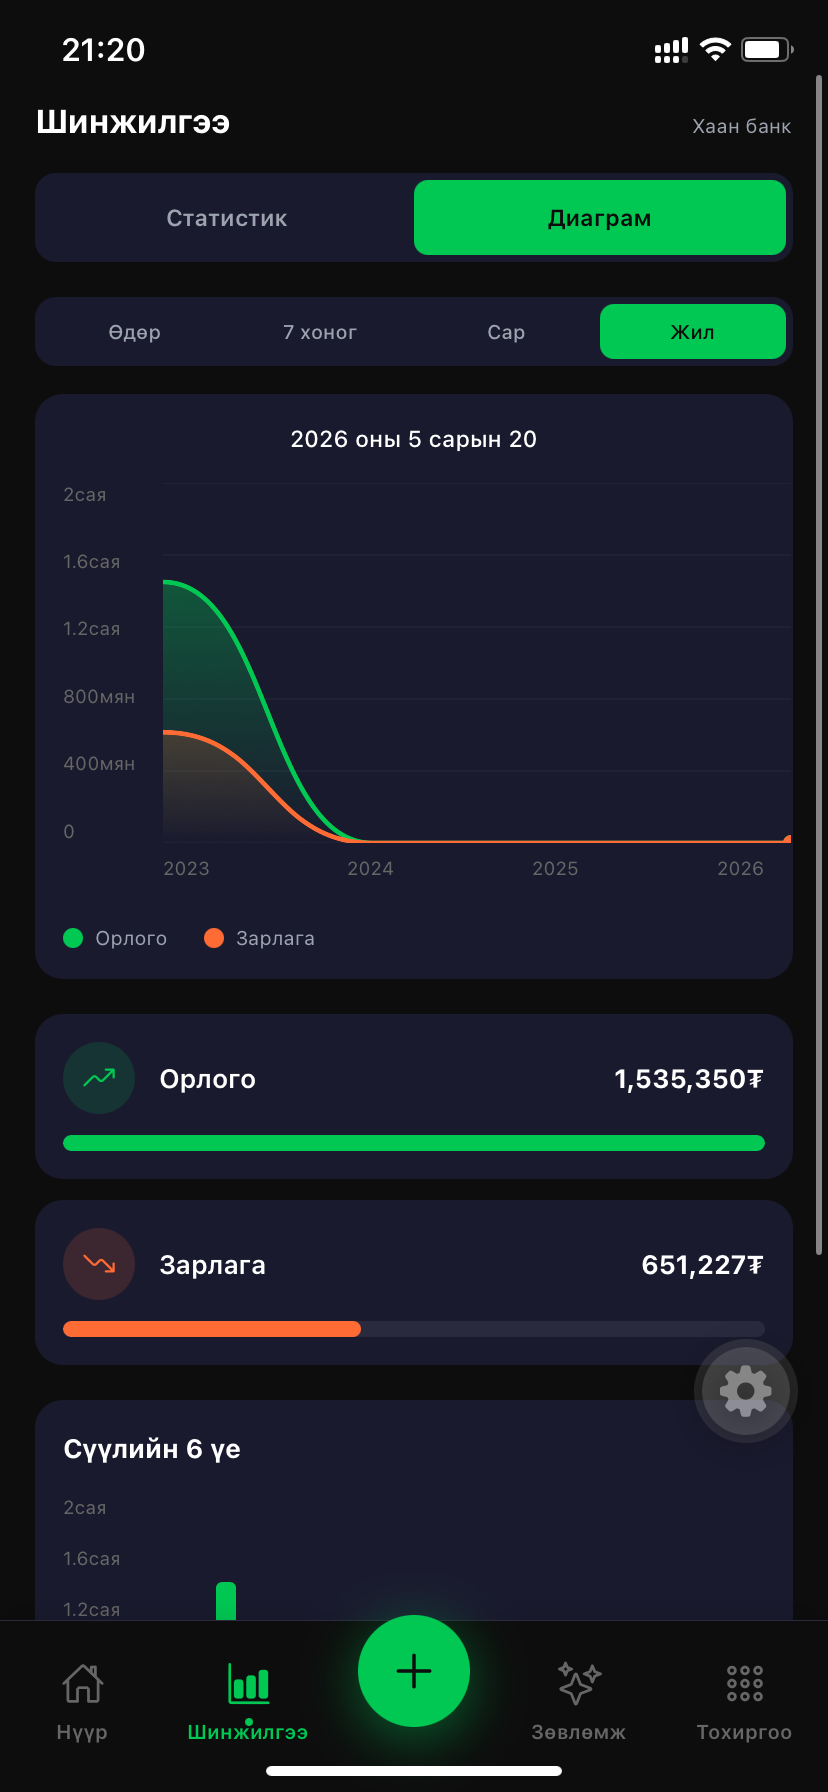
\includegraphics[width=\textwidth]{Figures/screen_chart_year_khan.png}
    \caption{Жил --- Хаан банк (2023--2026)}
    \label{fig:chart-year-khan}
\end{subfigure}
\caption{Диаграмм горим --- орлого, зарлагын чиг хандлагын муруй}
\label{fig:chart-screens}
\end{figure}

\textbf{Гол элементүүд:}
\begin{itemize}
    \item \textbf{Огноо толгой.} График дээр харагдах огноо (2026 оны 5 сарын 20).
    \item \textbf{Хугацааны тэнхлэг.} Өдөр, долоо хоног, сар, жилийн шүүлтүүрээс шалтгаалан тэнхлэгийн утга өөрчлөгдөнө.
    \item \textbf{Тунгалаг бүрхүүл.} Муруйн доорх талбар нь өнгөөр сүүдэрлэгдсэн тул орлого, зарлагын хэмжээг нүдээр амархан харьцуулна.
    \item \textbf{Орлого ба зарлагын явцын зурвас.} Орлого 7{,}491{,}834 төг, зарлага 7{,}698{,}944 төг-тэй харьцуулалт.
    \item \textbf{Хосолсон тэнхлэг.} Зүүн талын тэнхлэг сая, мянган нэгжтэй автомат форматтай.
\end{itemize}

\textbf{Ар талын логик.} \texttt{GET /api/v1/expenses/summary} болон \texttt{GET /api/v1/statistics} нь нэг хүсэлтэд багтаагдана. Хэрэглэгч тал нь \texttt{react-native-svg}-ийн \texttt{Polyline} болон Path-ыг ашиглан Bezier муруйгаар жигд интерполяц хийнэ.

\section{AI Зөвлөмж --- Чат хэсэг}
Систем дэх хамгийн онцлог дэлгэцүүдийн нэг бол \textbf{AI санхүүгийн зөвлөгч} юм. Хэрэглэгч хувийн санхүүгийн чөлөөт асуултаа бичиж, бодит мэдээлэл дээрээ үндэслэсэн зөвлөгөө авдаг. Чат хэсэг гурван үе шаттай ажиллана: эхлэлийн дэлгэц, асуулт бичсэн төлөв, AI хариу.

\begin{figure}[H]
\centering
\begin{subfigure}[t]{0.28\textwidth}
    \centering
    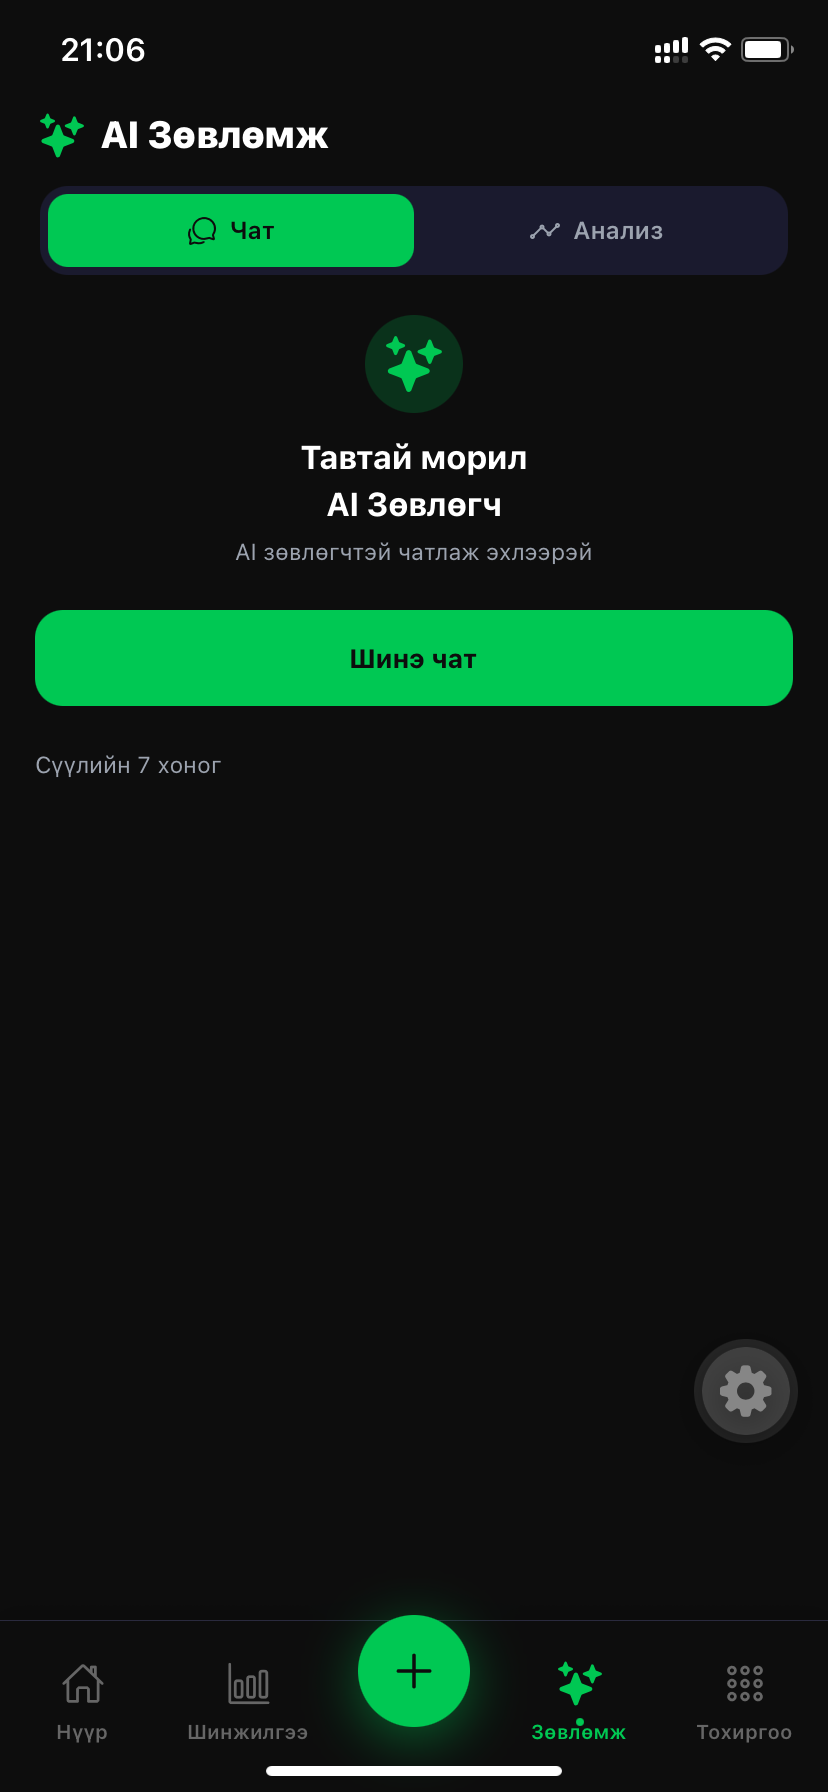
\includegraphics[width=\textwidth]{Figures/screen_ai_chat_start.png}
    \caption{Шинэ чат эхлүүлэх}
    \label{fig:ai-chat-start}
\end{subfigure}
\hfill
\begin{subfigure}[t]{0.28\textwidth}
    \centering
    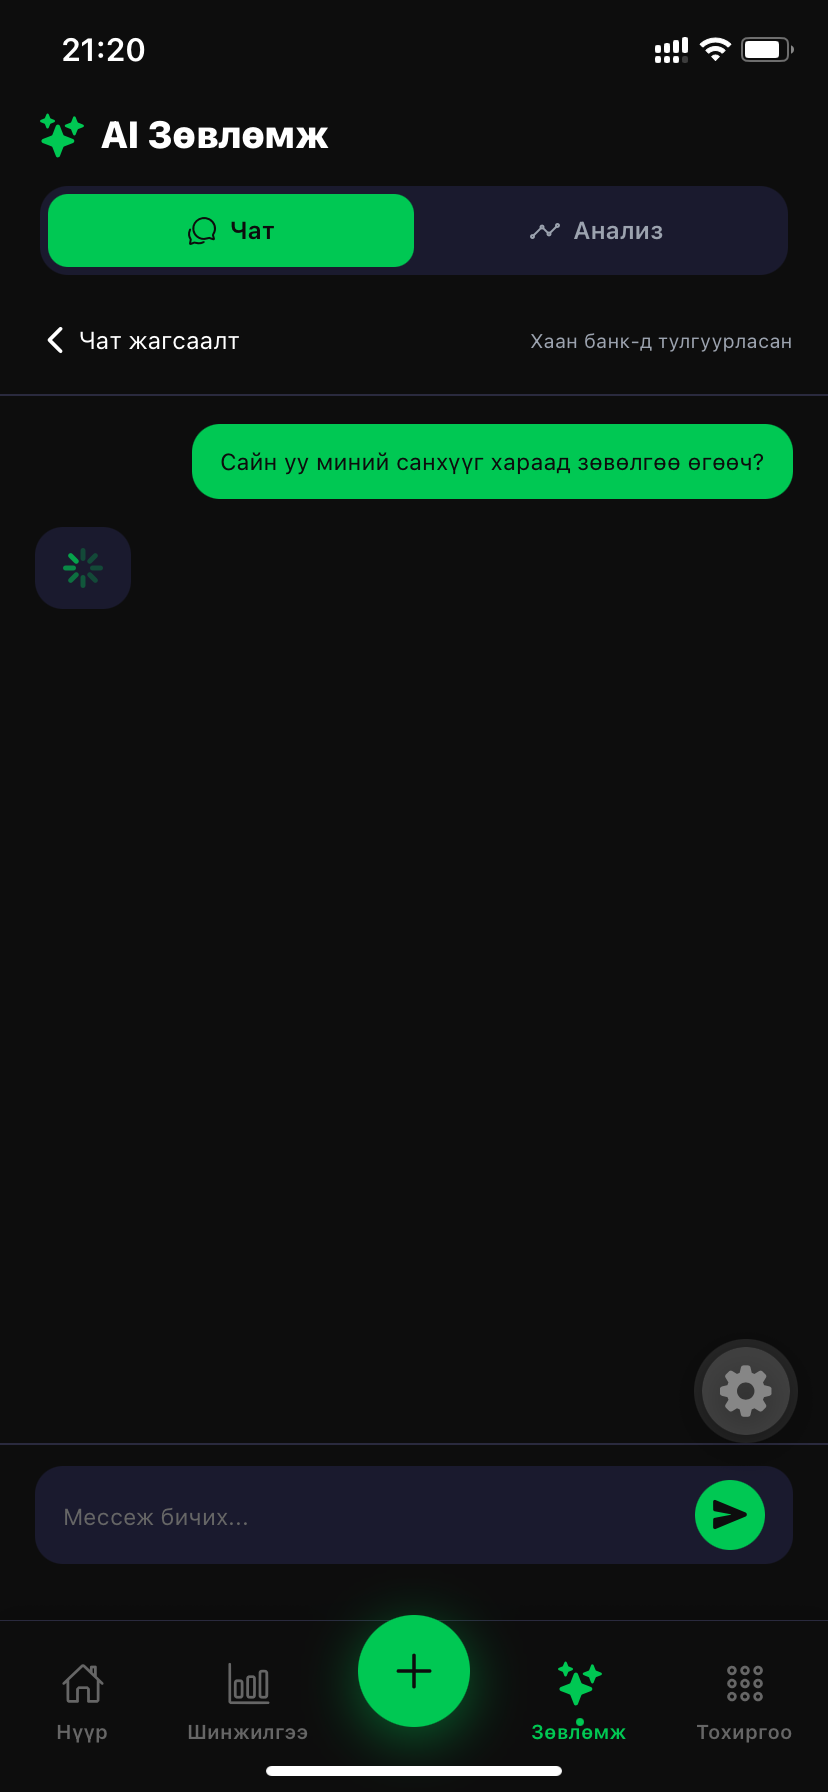
\includegraphics[width=\textwidth]{Figures/screen_ai_chat_empty.png}
    \caption{Асуулт бичих}
    \label{fig:ai-chat-empty}
\end{subfigure}
\hfill
\begin{subfigure}[t]{0.28\textwidth}
    \centering
    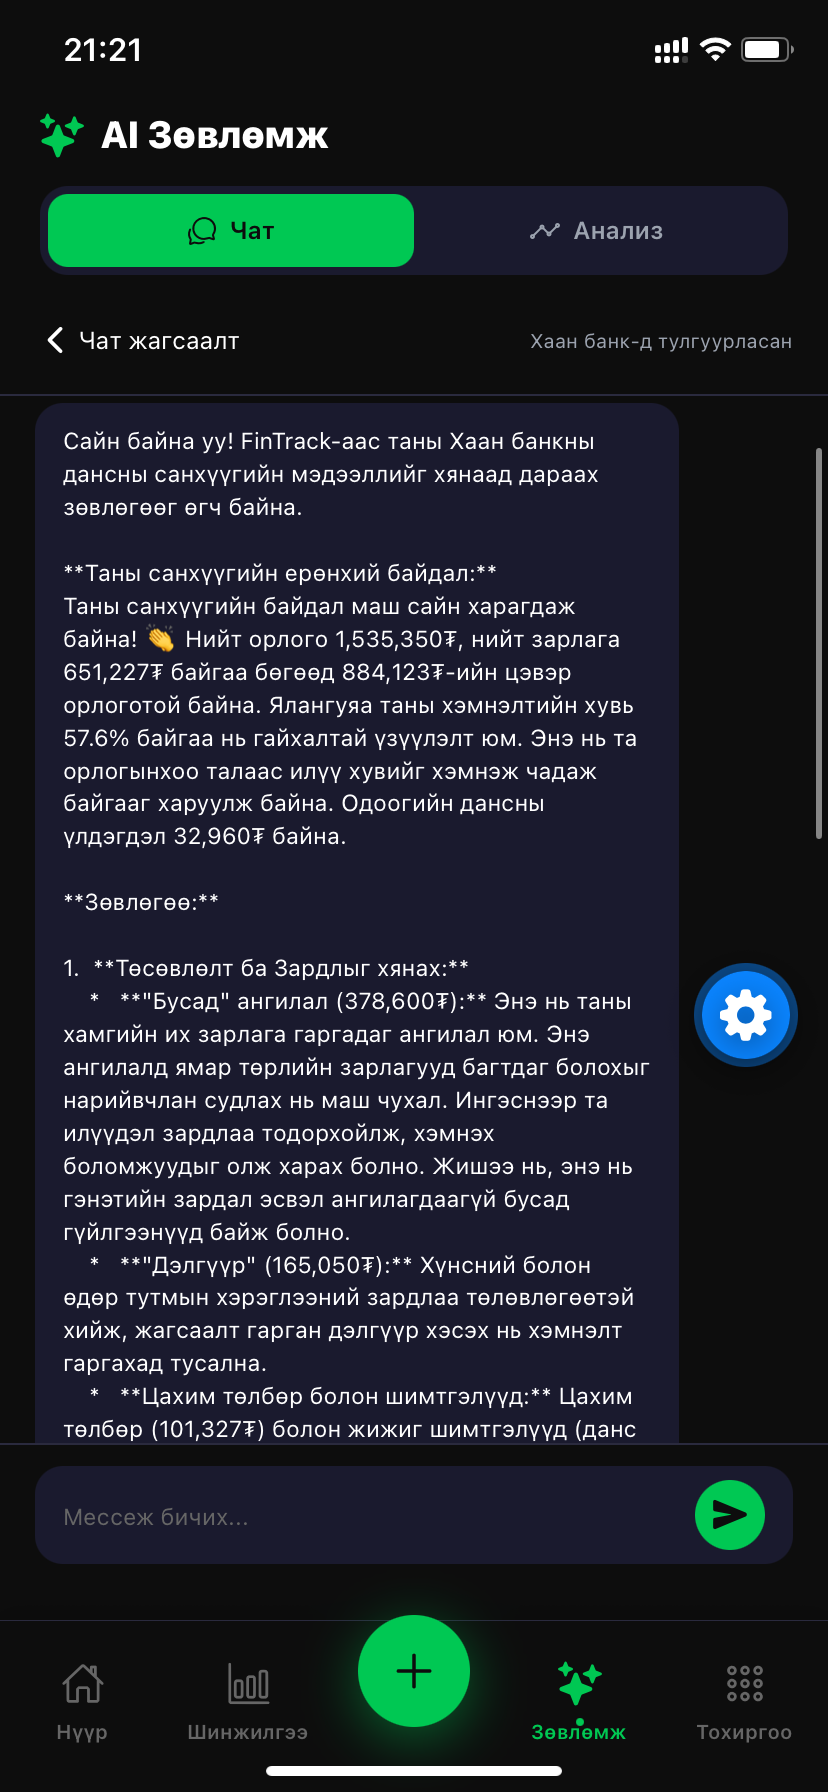
\includegraphics[width=\textwidth]{Figures/screen_ai_chat_response.png}
    \caption{AI зөвлөгөө буцаах}
    \label{fig:ai-chat-response}
\end{subfigure}
\caption{AI санхүүгийн зөвлөгчтэй чатлах гурван үе шат}
\label{fig:ai-chat}
\end{figure}

\textbf{Зургийн жишээ агуулга.} Хэрэглэгч "\textit{Сайн уу, миний санхүүг хараад зөвлөгөө өгөөч?}" гэж асуухад AI:
\begin{itemize}
    \item Бодит мэдээллээ дурдаж \textbf{одоогийн санхүүгийн байдлын тойм} гаргана: нийт орлого 1{,}535{,}350 төг, нийт зарлага 651{,}227 төг, цэвэр орлого 884{,}123 төг, хэмнэлтийн хувь 57.6\%, одоогийн дансны үлдэгдэл 32{,}960 төг.
    \item \textbf{Бүтэцлэгдсэн зөвлөмж} буцаадаг: төсөвлөлт ба зардлыг хянах, "Бусад" ангиллыг нарийвчлан судлах, цахим төлбөр ба шимтгэлийг бууруулах гэх мэт.
    \item Тоон жишээ ашиглан тодорхой санал болгоно.
\end{itemize}

\textbf{Ар талын логик.} \texttt{POST /api/v1/ai/chat} нь \texttt{ai\_chat.go:SendMessage} боловсруулагчийг ажиллуулна. Энэ боловсруулагч нь:
\begin{enumerate}
    \item Одоогийн хэрэглэгчийн сүүлийн \textbf{30 хоногийн гүйлгээг} өгөгдлийн сангаас цуглуулна,
    \item Бүх дансны нийт үлдэгдлийг тооцоолно,
    \item Ангилал тус бүрийн нийт зарлагыг гаргана,
    \item Энэ нэгдсэн контекстийг JSON хэлбэрээр системийн зааварчилгаанд нэмж, хэрэглэгчийн асуултыг хэрэглэгчийн зааварчилгаа болгоно,
    \item Олон нийлүүлэгчтэй AI давхарга (\texttt{ai\_provider.go}) руу контекст бэлтгэн илгээж, үндсэн \texttt{gemini-2.5-flash} болон OpenRouter-ийн нөөц загваруудыг ашиглана.
    \item Чатын түүхийг \texttt{ai\_messages} хүснэгтэд хадгална.
\end{enumerate}

\section{AI Зөвлөмж --- Шинжилгээний хэсэг}
Шинжилгээний хэсэг нь хэрэглэгч банкны хуулгаа байршуулсны дараа эсвэл өдөр тутмын автомат шинжилгээний үр дүнг харуулдаг. Энэ нь чат хэлбэрээс ялгаатай нь \emph{бүтэцлэгдсэн} (structured) форматтай, олон үе шаттай: хуулга байршуулах, шинжилгээний нэгтгэл, дэлгэрэнгүй зөвлөмж, гүйлгээний бүрэн жагсаалт.

\begin{figure}[H]
\centering
\begin{subfigure}[t]{0.28\textwidth}
    \centering
    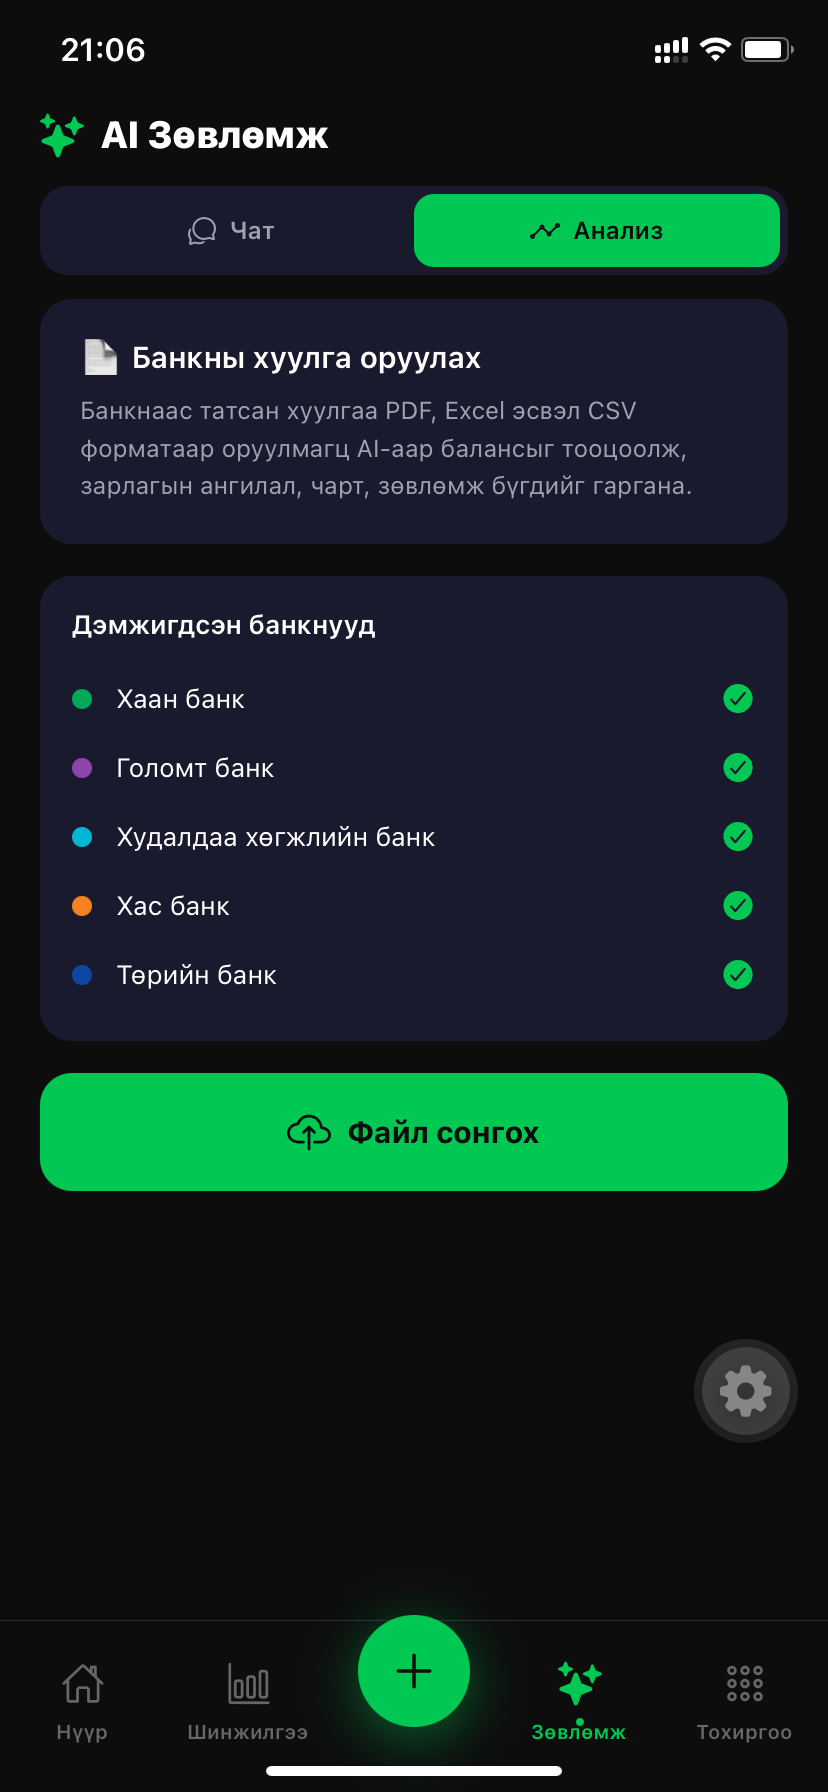
\includegraphics[width=\textwidth]{Figures/screen_ai_upload.png}
    \caption{Хуулга оруулах}
    \label{fig:ai-upload}
\end{subfigure}
\hfill
\begin{subfigure}[t]{0.28\textwidth}
    \centering
    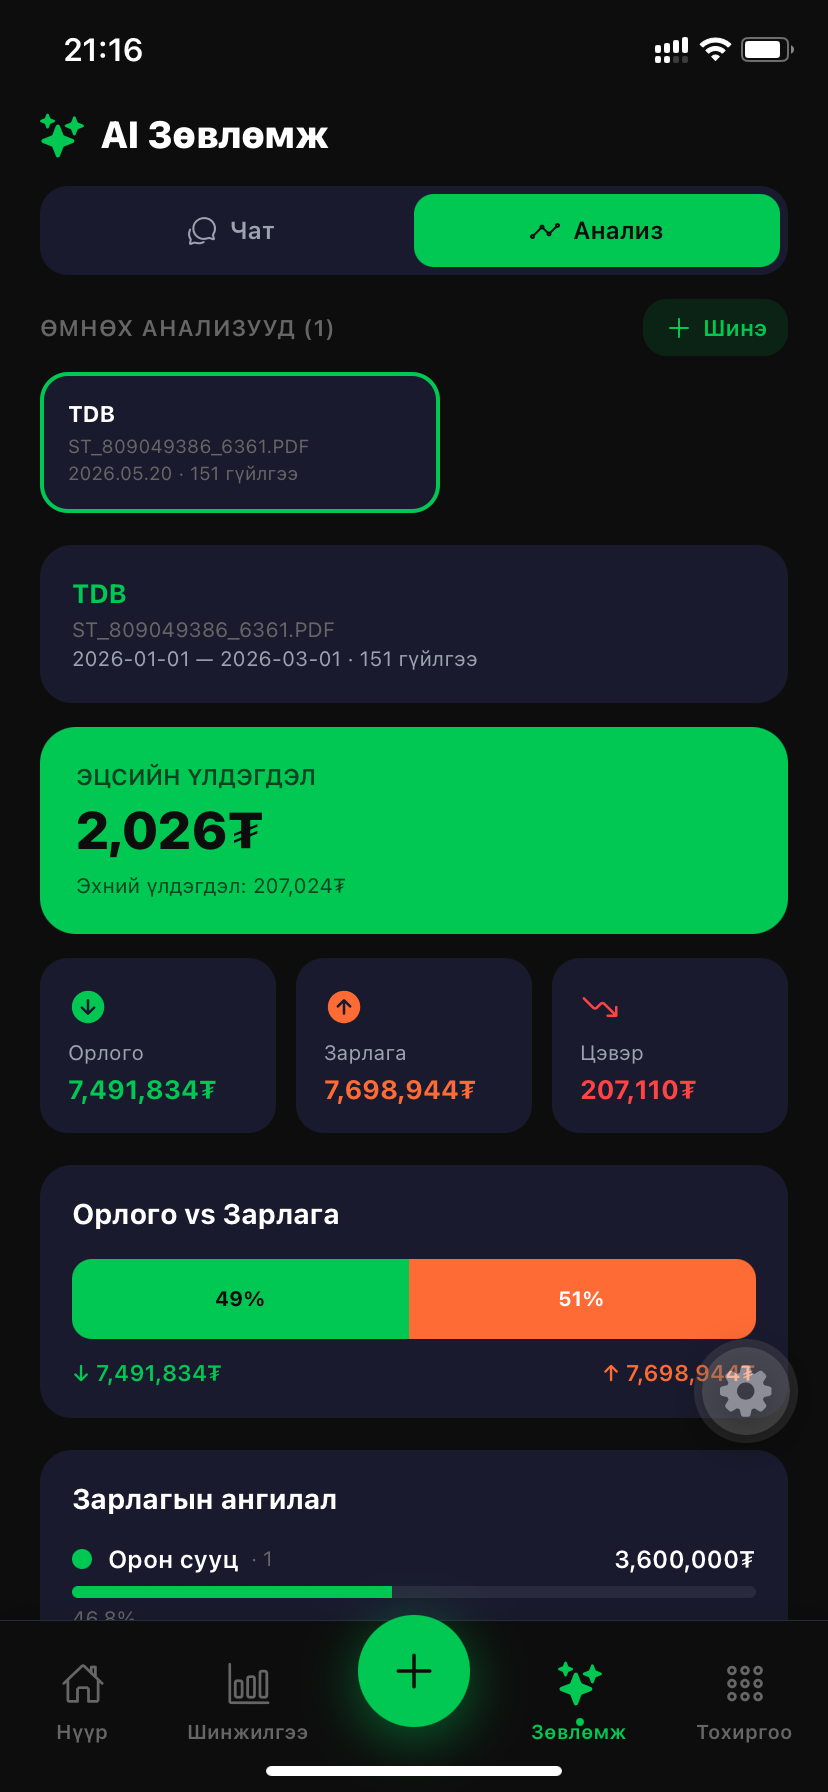
\includegraphics[width=\textwidth]{Figures/screen_ai_analysis_tdb.png}
    \caption{TDB шинжилгээ}
    \label{fig:ai-analysis-tdb}
\end{subfigure}
\hfill
\begin{subfigure}[t]{0.28\textwidth}
    \centering
    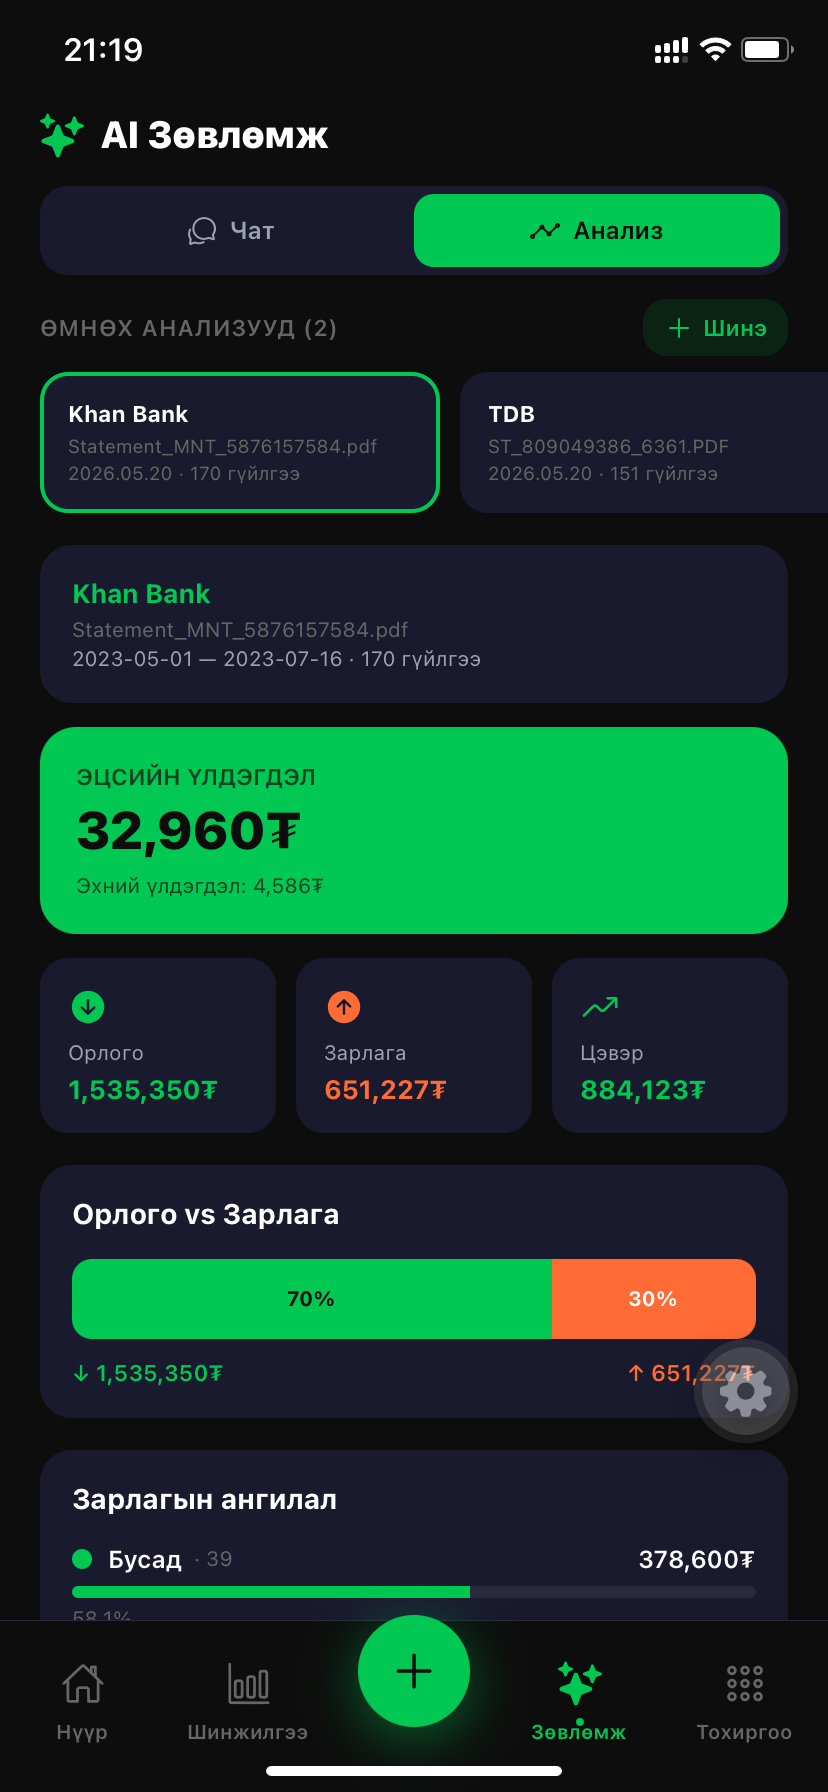
\includegraphics[width=\textwidth]{Figures/screen_ai_analysis_khan.png}
    \caption{Хаан банк шинжилгээ}
    \label{fig:ai-analysis-khan}
\end{subfigure}
\caption{Банкны хуулгын AI шинжилгээний гурван дэлгэц}
\label{fig:ai-analysis}
\end{figure}

\textbf{Хуулга байршуулах дэлгэц} нь дэмжигдсэн 5 банкны жагсаалт (Хаан банк, Голомт банк, Худалдаа хөгжлийн банк, Хас банк, Төрийн банк)-тай. Хэрэглэгч PDF, Excel эсвэл CSV форматын файл сонгож байршуулна.

\textbf{Шинжилгээний нэгтгэл дэлгэц} нь хуулга боловсруулагдсаны дараа дараах мэдээллийг харуулдаг:
\begin{itemize}
    \item \textbf{Өмнөх шинжилгээний карт.} Хэрэглэгч хэд хэдэн хуулга байршуулсан байвал жижиг картаар жагсаана. Идэвхтэй сонголт нь ногоон хүрээтэй.
    \item \textbf{Дансны мэдээлэл.} Банкны нэр, файлын нэр, огнооны хүрээ, гүйлгээний тоо.
    \item \textbf{Эцсийн үлдэгдэл.} Том ногоон карт дээр хуулгын эцсийн үлдэгдэл (Хаан банк --- 32{,}960 төг, TDB --- 2{,}026 төг).
    \item \textbf{Орлого/Зарлага/Цэвэр.} 3 жижиг карт дээр нэгтгэл.
    \item \textbf{Орлого ба зарлага.} Хувийн харьцааг нэг урт явцын зурвасаар (Хаан банк дээр 70/30, TDB дээр 49/51).
    \item \textbf{Зарлагын ангилал.} Хамгийн их зарлагатай ангиллууд тоо, мөнгөн дүн, хувийн жинтэйгээр.
\end{itemize}

\subsection{Дэлгэрэнгүй AI зөвлөмж ба гүйлгээний жагсаалт}
Шинжилгээний нэгтгэлийг доош гүйлгэхэд AI-ийн дэлгэрэнгүй зөвлөмж ба бүх гүйлгээний жагсаалт гарна.

\begin{figure}[H]
\centering
\begin{subfigure}[t]{0.36\textwidth}
    \centering
    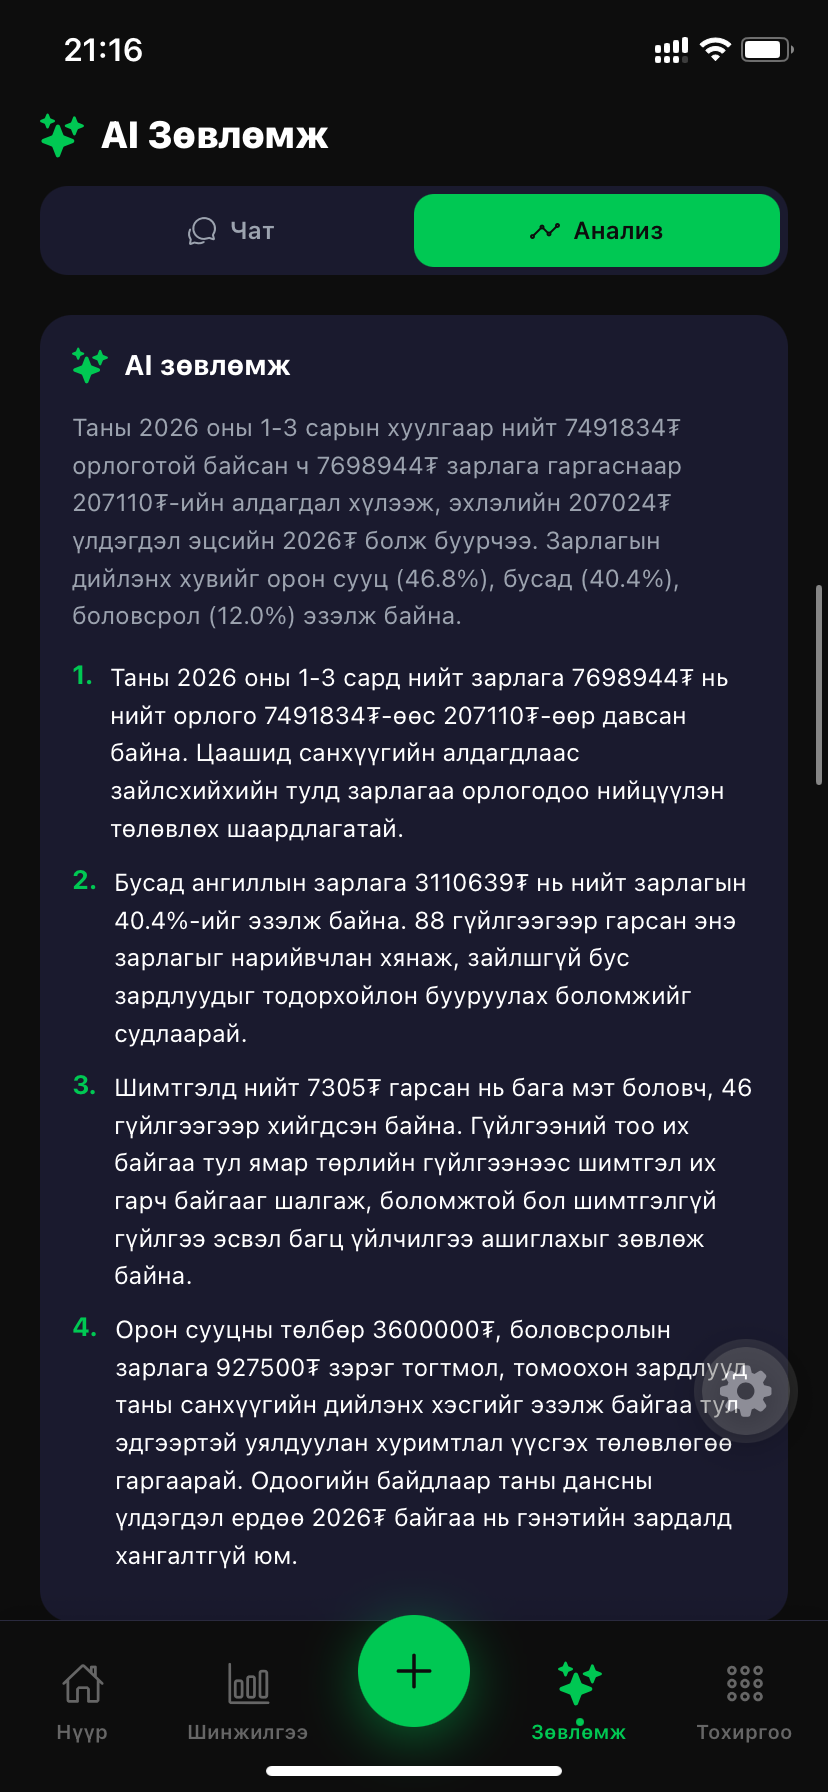
\includegraphics[width=\textwidth]{Figures/screen_ai_rec_detail.png}
    \caption{Дэлгэрэнгүй AI зөвлөмж}
    \label{fig:ai-rec-detail}
\end{subfigure}
\hfill
\begin{subfigure}[t]{0.36\textwidth}
    \centering
    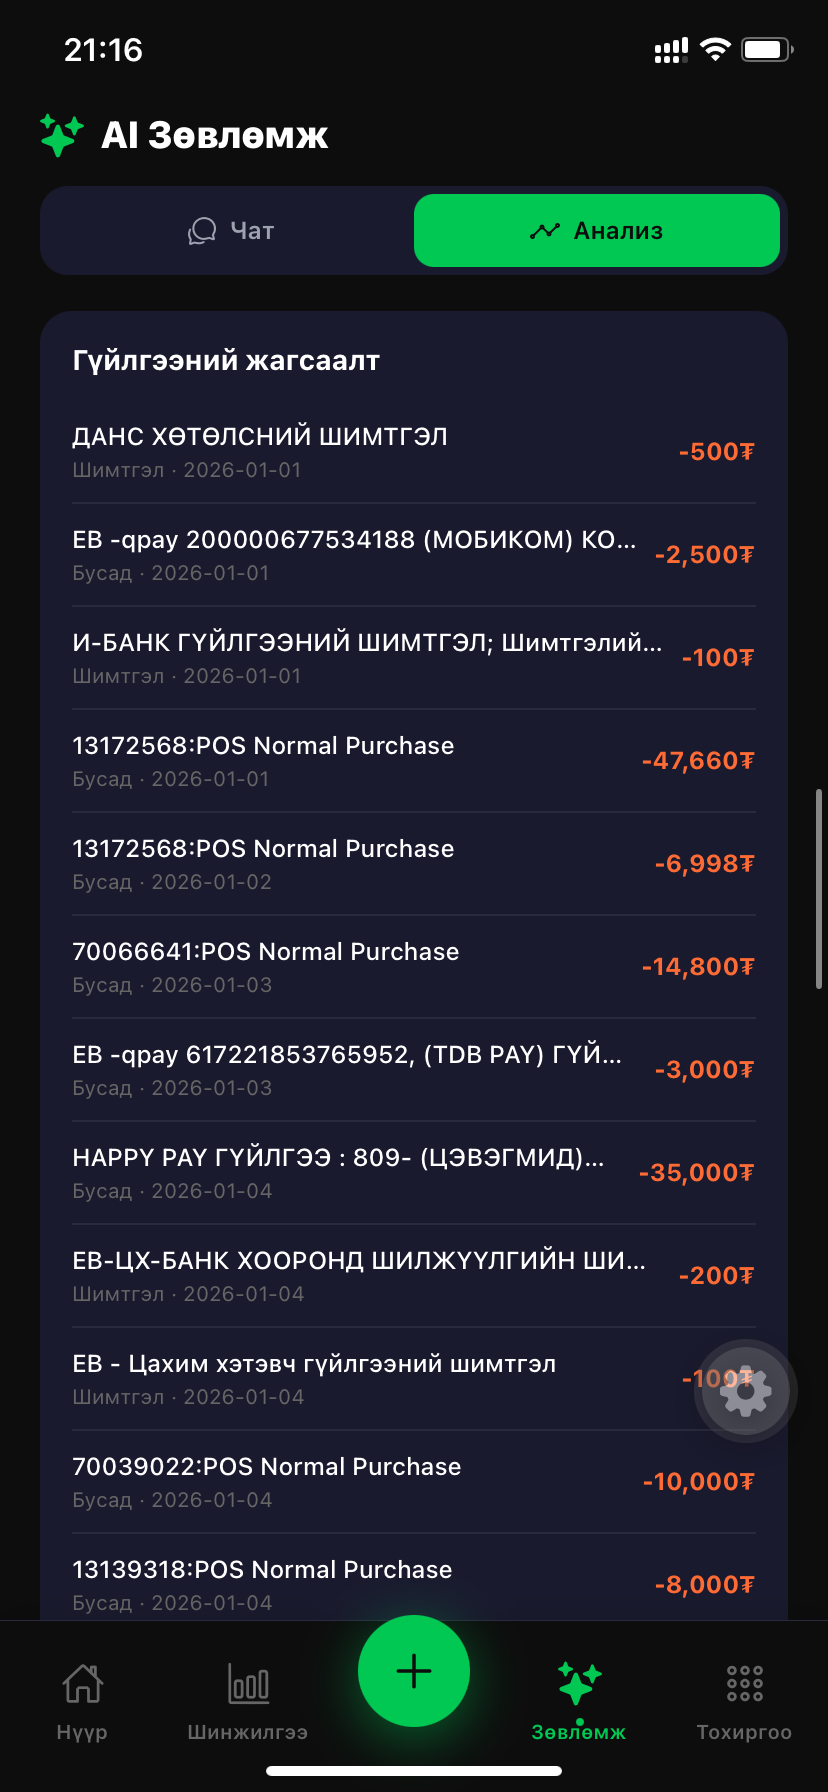
\includegraphics[width=\textwidth]{Figures/screen_ai_transactions.png}
    \caption{Гүйлгээний жагсаалт}
    \label{fig:ai-transactions}
\end{subfigure}
\caption{AI зөвлөмжийн дэлгэрэнгүй ба боловсруулсан гүйлгээний жагсаалт}
\label{fig:ai-rec-tx}
\end{figure}

AI зөвлөмжийн картад тоон үндэслэлтэй дугаарлагдсан зөвлөмж 4-6 эгнээ багтдаг. Жишээ нь "Таны 2026 оны 1-3 сард нийт зарлага 7{,}698{,}944 төг нь нийт орлого 7{,}491{,}834 төг-өөс 207{,}110 төг-өөр давсан байна" гэх мэт хатуу тоонд тулгуурласан санал гаргадаг.

Гүйлгээний жагсаалт нь хуулгаас уншигдсан бүх гүйлгээг ангилалтайгаар нь харуулна. Гүйлгээ бүрд тайлбар, ангилал, огноо, дүн харагдана.

\textbf{Ар талын логик.} \texttt{POST /api/v1/ai/analysis}-аар банкны хуулга байршуулсны дараа \texttt{ai\_analysis.go} боловсруулагчийн \texttt{generateAIInsights} функц ажиллана. Задлан уншсан гүйлгээний жагсаалт, ангилал, орлого, зарлагын нэгтгэлийг JSON хэлбэрээр LLM рүү илгээж, гарч ирсэн 3-5 хэрэгжих зөвлөмжийг буцаан авдаг. Үр дүнг \texttt{ai\_analyses.recommendations\_json} баганад хадгална.

\section{Давтагдах төлбөр}
Хэрэглэгч сар бүр байнга төлдөг тогтмол төлбөрөө (Netflix, утасны төлбөр, зээлийн эргэн төлөлт гэх мэт) урьдчилан тохируулах боломжтой. Дэлгэц нь хоосон төлөвөөс эхлэн \texttt{+} товчлуурын тусламжтайгаар нэмэгддэг.

\begin{figure}[H]
\centering

\includegraphics[width=0.36\textwidth]{Figures/screen_scheduled_empty.png}
\caption{Давтагдах төлбөр --- хоосон төлөвийн харагдац}
\label{fig:scheduled-empty}
\end{figure}

\textbf{Гол элементүүд:}
\begin{itemize}
    \item \textbf{Хоосон төлөвийн дүрс.} Хоёр сум эргэлт хийсэн дугуй дүрс, доор нь "Төлөвлөсөн төлбөр байхгүй" гэсэн заавар.
    \item \textbf{"Төлбөр нэмэх" товчлуур.} Гол үйлдлийн товчлуур нь ягаан өнгөтэй.
    \item \textbf{Шинэ нэмэх товчлуур.} Баруун дээд буланд \texttt{+} хэлбэртэй ягаан товчлуур.
\end{itemize}

\textbf{Ар талын логик.} \texttt{GET /api/v1/scheduled-payments} хариу нь хоосон жагсаалт буцаахад UI хоосон төлөвийг харуулна. Шинэ төлбөр нэмэхэд \texttt{POST /api/v1/scheduled-payments} руу \texttt{frequency} (daily, weekly, monthly, yearly), \texttt{next\_date} зэрэг талбарууд илгээгдэнэ.

\section{Тохиргооны дэлгэцүүд}
Тохиргооны бүлэг нь профайл, нууцлал, харагдац гэсэн гурван үндсэн дэд дэлгэцтэй.

\begin{figure}[H]
\centering
\begin{subfigure}[t]{0.28\textwidth}
    \centering
    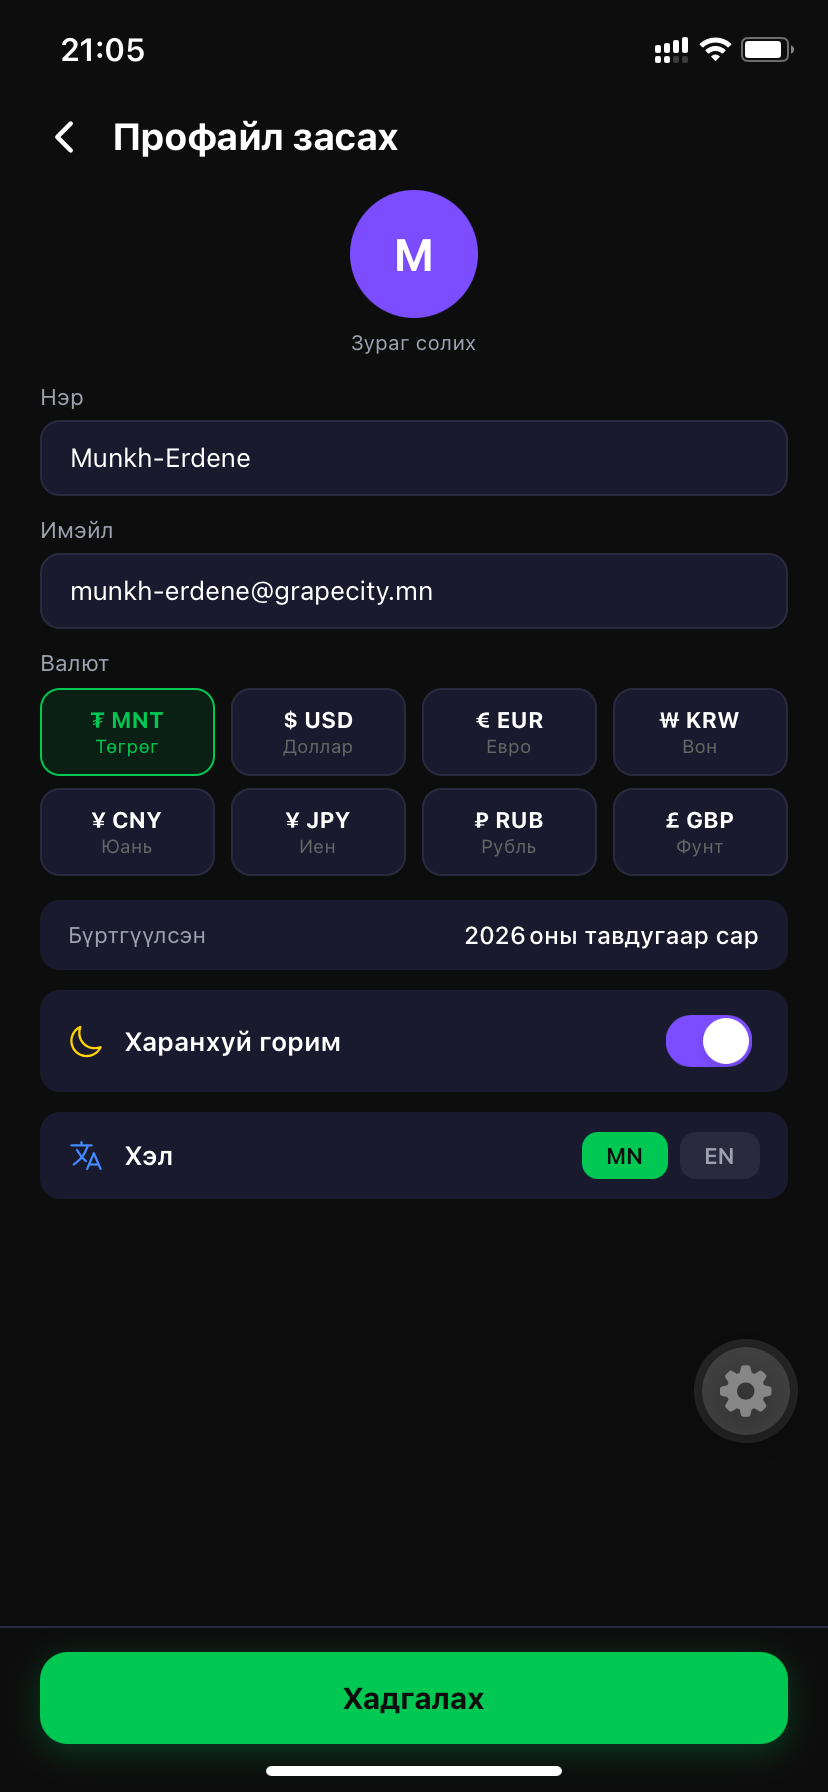
\includegraphics[width=\textwidth]{Figures/screen_profile.png}
    \caption{Профайл засах}
    \label{fig:profile}
\end{subfigure}
\hfill
\begin{subfigure}[t]{0.28\textwidth}
    \centering
    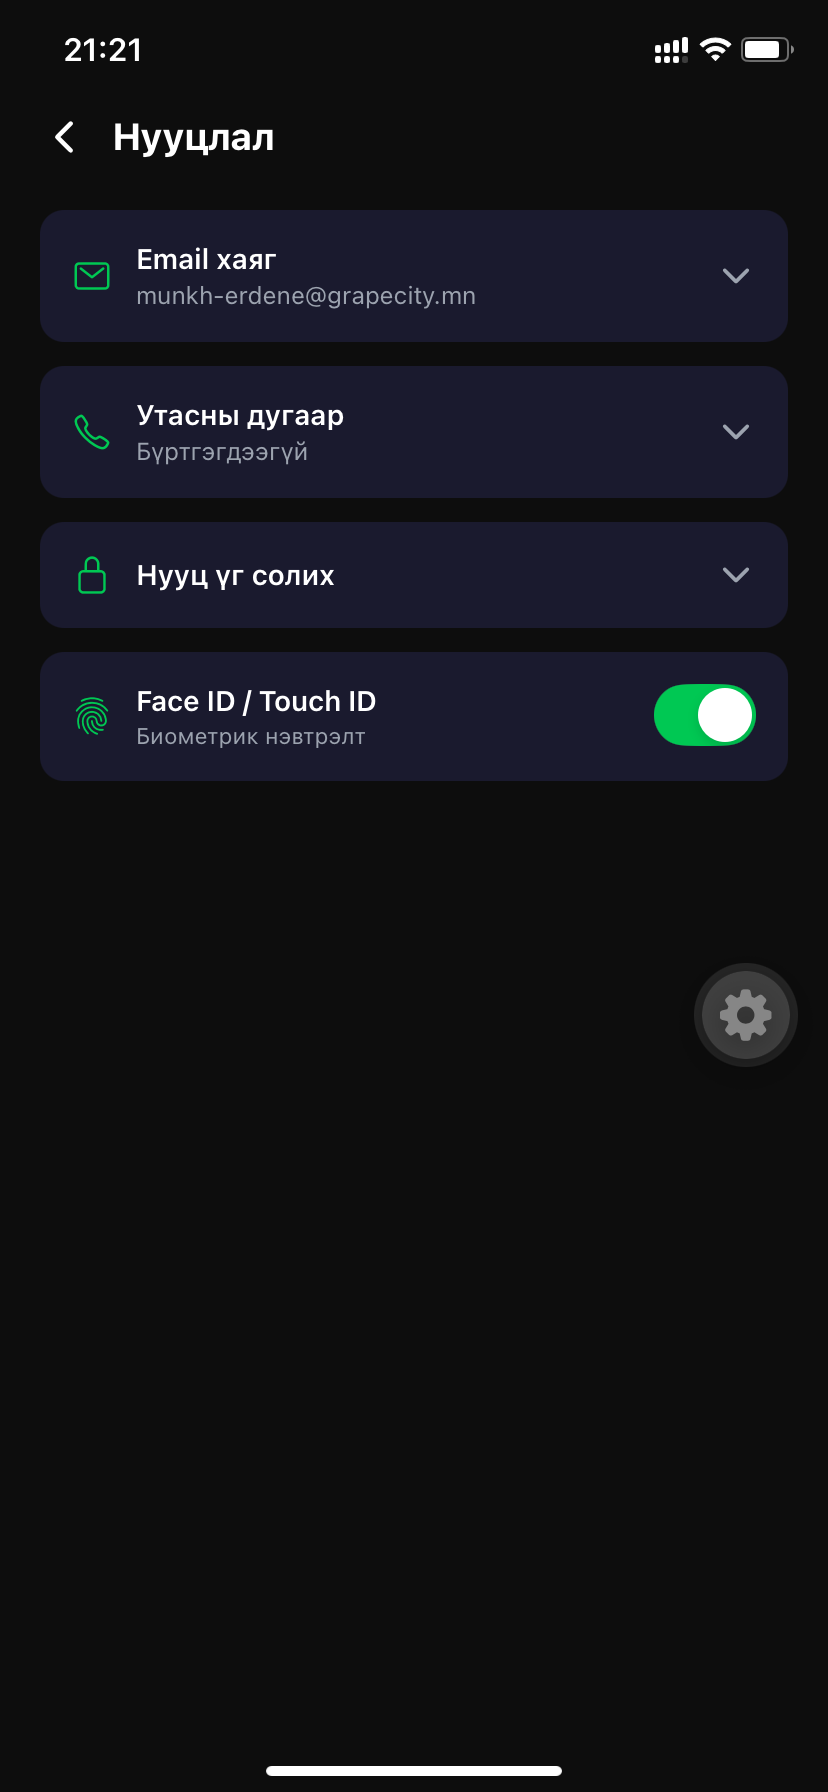
\includegraphics[width=\textwidth]{Figures/screen_privacy.png}
    \caption{Нууцлал}
    \label{fig:privacy}
\end{subfigure}
\hfill
\begin{subfigure}[t]{0.28\textwidth}
    \centering
    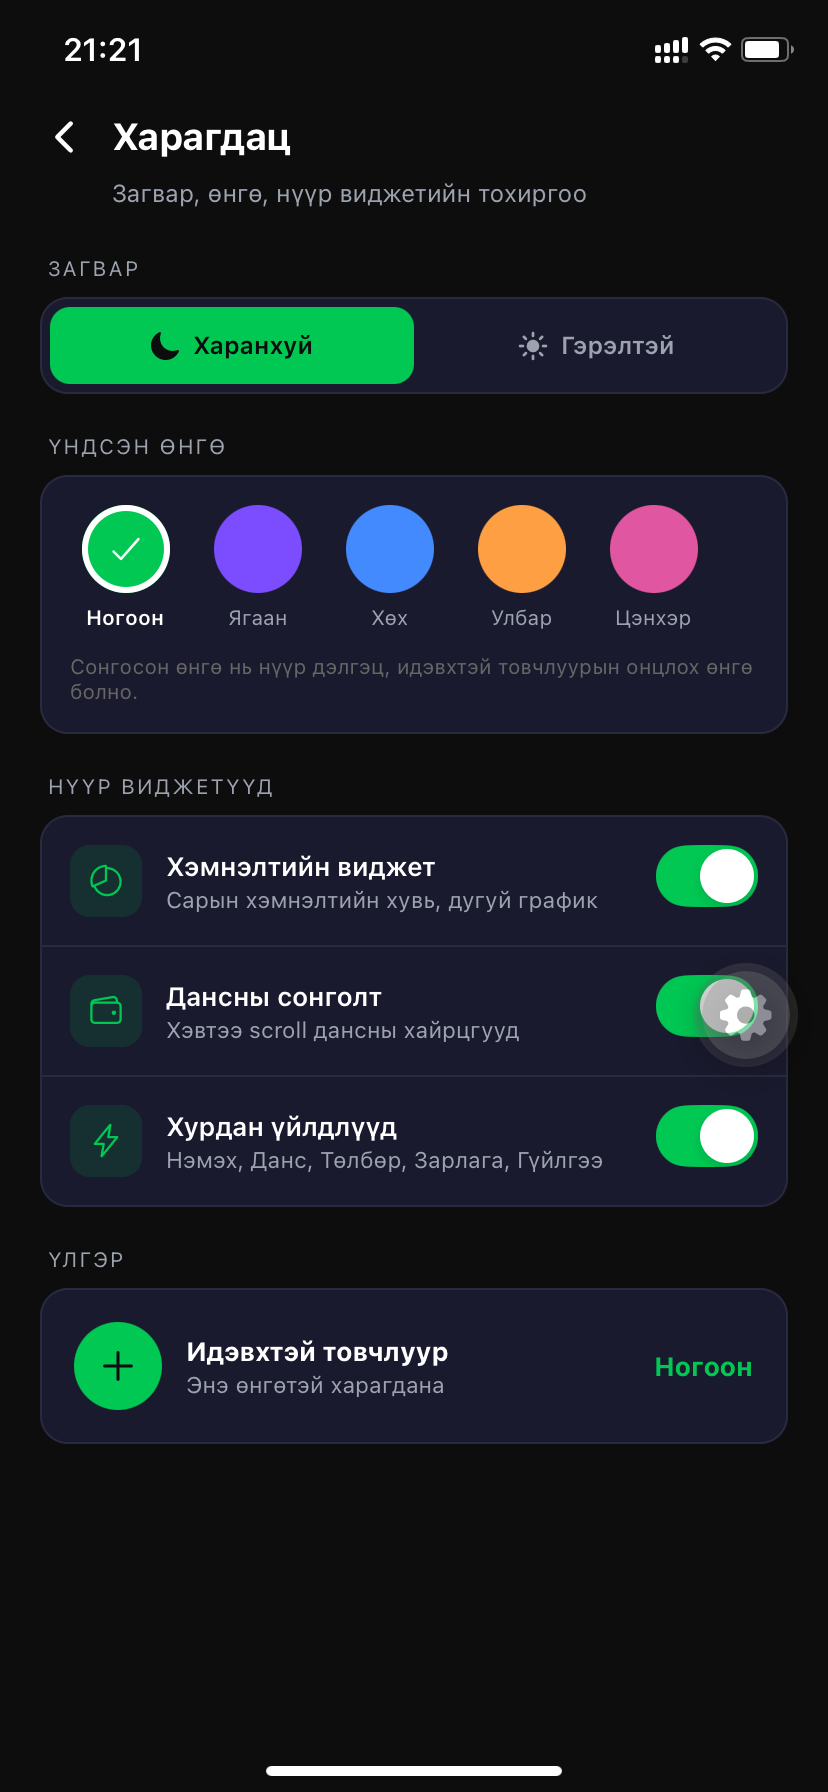
\includegraphics[width=\textwidth]{Figures/screen_display.png}
    \caption{Харагдац}
    \label{fig:display}
\end{subfigure}
\caption{Тохиргооны дэд дэлгэцүүд --- профайл, нууцлал, харагдац}
\label{fig:settings-screens}
\end{figure}

\textbf{Профайл засах} дэлгэц дээр хэрэглэгч өөрийн нэр, имэйл, валют, аватар зураг, харанхуй горим, программын хэлийг тохируулна. Дэмжигдэх валютууд: MNT (төгрөг), USD, EUR, KRW, CNY, JPY, RUB, GBP гэсэн 8 валют. Сонгосон валют ногоон хүрээтэй болно. Хэлний сонголтод MN/EN гэсэн 2 сонголт байна.

\textbf{Нууцлал} дэлгэц дээр имэйл хаяг, утасны дугаар харуулах, нууц үг солих, Face ID / Touch ID-аар нэвтрэх сонголт тус бүрийг дэлгэгддэг хэсэг хэлбэрээр зохион байгуулсан.

\textbf{Харагдац} дэлгэц нь программын дүр төрхийг өөрчилнө:
\begin{itemize}
    \item \textbf{Загвар.} Харанхуй (анхдагч) ба гэрэлтэй гэсэн хоёр сонголт.
    \item \textbf{Үндсэн өнгө.} Ногоон (анхдагч), Ягаан, Хөх, Улбар, Цэнхэр гэсэн 5 өнгө. Сонгосон өнгө нь нүүр дэлгэц болон идэвхтэй товчлууруудын онцлох өнгөнд хэрэглэгдэнэ.
    \item \textbf{Нүүр виджетүүд.} Хэрэглэгч хэмнэлтийн виджет, дансны сонголт, хурдан үйлдлүүдийг асааж / унтрааж болно.
    \item \textbf{Үлгэр.} Сонгосон тохиргооны жишээ урьдчилан харах хэсэг.
\end{itemize}

\textbf{Ар талын логик.} \texttt{PUT /api/v1/profile} (нэр, имэйл, валют) ба \texttt{POST /api/v1/profile/avatar} (зураг multipart) гэсэн API цэгүүдээр хэрэглэгчийн өгөгдлийг шинэчилнэ. Тохиргооны сонголтууд (theme, color, widgets) нь \texttt{AsyncStorage}-д локалаар хадгалагдан, серверт \texttt{PUT /api/v1/preferences}-ээр синхрончлогдоно.

\section{Push мэдэгдэл}
Систем Expo Push Notifications үйлчилгээг ашиглан хэрэглэгчид санхүүгийн анхааруулга илгээдэг. Push мэдэгдэл нь өргөн хүрээний нөхцөлд хэрэгжинэ: зарлага орлогоос хэтрэх, давтагдах төлбөр сануулах, AI-ийн өдөр тутмын дүгнэлт, цаг бүрийн эрсдэлийн анхааруулга гэх мэт.

\begin{figure}[H]
\centering
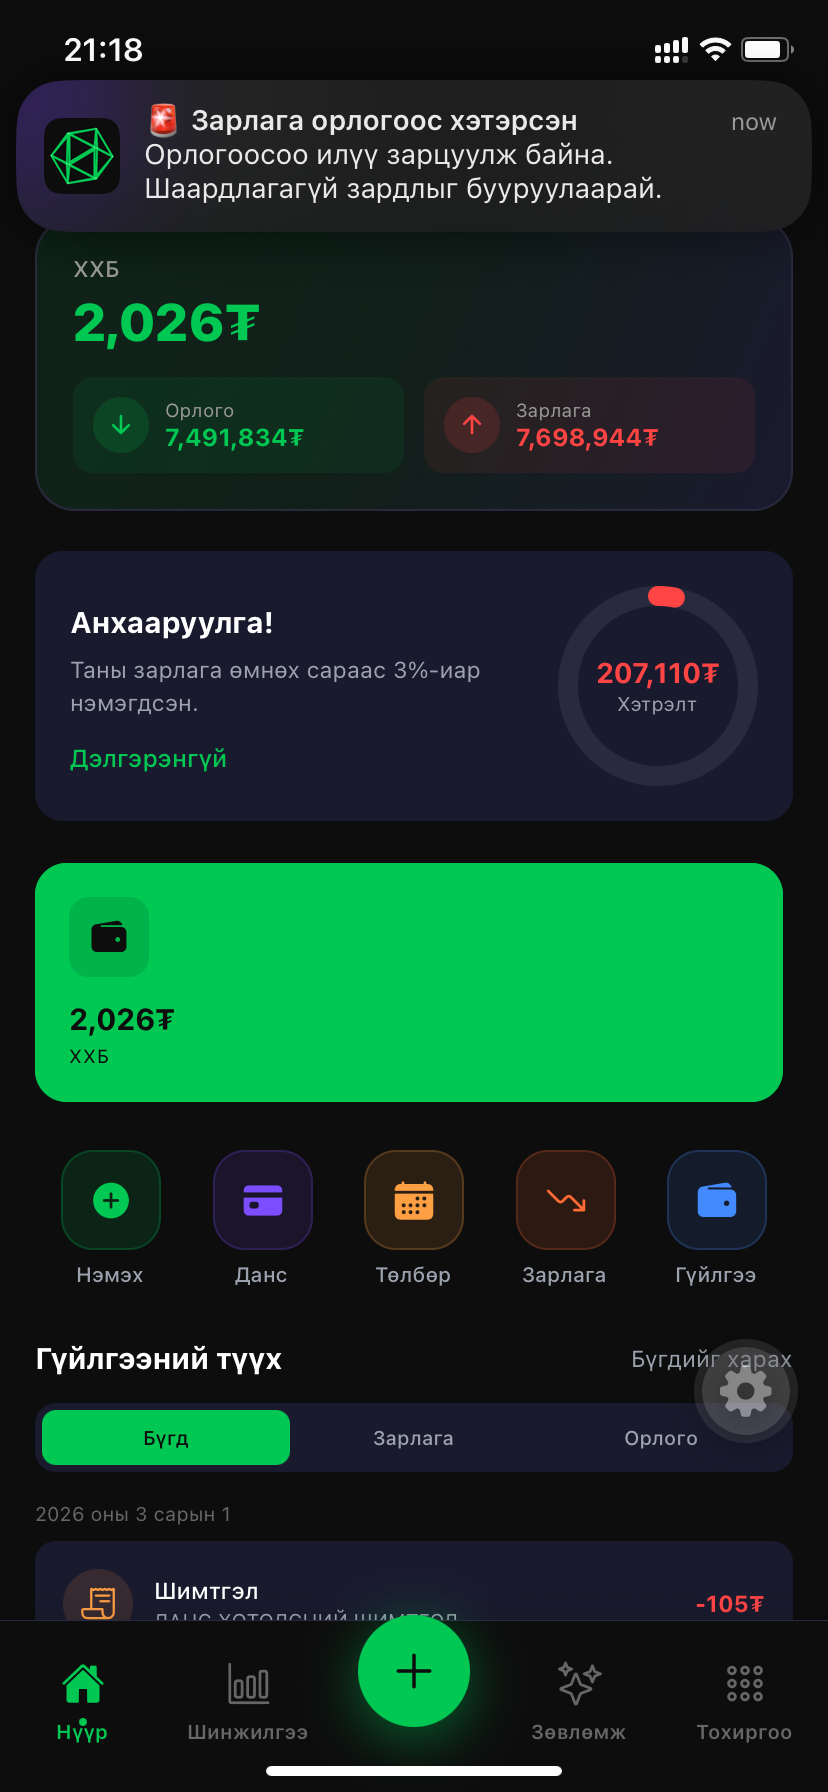
\includegraphics[width=0.36\textwidth]{Figures/screen_push_notification.png}
\caption{Push мэдэгдэл --- зарлага орлогоос хэтэрсэн анхааруулга}
\label{fig:push}
\end{figure}

\textbf{Жишээ.} Зурагт "Зарлага орлогоос хэтэрсэн --- Орлогоосоо илүү зарцуулж байна. Шаардлагагүй зардлыг бууруулаарай." гэсэн мэдэгдэл харагдаж байна. Хэрэглэгч уг мэдэгдэл дээр дарвал нүүр дэлгэц рүү шилжих эсвэл шинжилгээний хуудас руу очно.

\textbf{Ар талын логик.} Гар утасны программ анх ачаалахад \texttt{expo-notifications} сангаар push токен авч \texttt{POST /api/v1/users/push-token} API цэг рүү илгээдэг. Сервер талд Go-ийн \texttt{robfig/cron} сан ашиглан өдөр бүр 21:00 цагт автомат ажиллагч ажиллана. Ажиллагч нь бүх идэвхтэй хэрэглэгчдийн сүүлийн 24 цагийн гүйлгээг шалгаж, шаардлагатай тохиолдолд Expo push API руу мэдэгдэл илгээнэ.

\section{Хэрэглэгчийн бодит хэрэглээний жишээ}
Дээрх дэлгэцүүдийн логик уялдааг бодит хэрэглэгчийн нэг өдрийн жишээгээр харуулъя.

\begin{table}[ht]
\centering
\footnotesize
\renewcommand{\arraystretch}{1.3}
\rowcolors{2}{softgrey}{white}
\begin{tabular}{|c|p{4cm}|p{8cm}|}
\hline
\rowcolor{darknavy}
\textcolor{white}{\textbf{Алхам}} & \textcolor{white}{\textbf{Үйлдэл}} & \textcolor{white}{\textbf{Дэлгэц / API}} \\ \hline
1 & Программ нээх             & Splash $\to$ Login $\to$ Home (\texttt{GET /dashboard}) \\ \hline
2 & Өглөөний цайны мөнгө бүртгэх & \texttt{+} товч $\to$ AddTx (\texttt{POST /transactions}) \\ \hline
3 & Дансаа шалгах             & Home $\to$ Хаан банкны карт сонгох \\ \hline
4 & Сарын зарлагаа харах      & Шинжилгээ $\to$ Сар (\texttt{GET /statistics?period=monthly}) \\ \hline
5 & AI-аас зөвлөгөө асуух     & Зөвлөмж таб $\to$ AI чат (\texttt{POST /ai/chat}) \\ \hline
6 & Сарын төлбөр нэмэх        & Тохиргоо $\to$ Давтагдах $\to$ \texttt{+} (\texttt{POST /scheduled-payments}) \\ \hline
7 & Банкны хуулга оруулах     & Тохиргоо $\to$ Хуулга $\to$ файл сонгох (\texttt{POST /ai/analysis}) \\ \hline
8 & Зөвлөмж унших             & Шинжилгээний үр дүн $\to$ AI зөвлөмж (\texttt{GET /ai/analyses/:id}) \\ \hline
\end{tabular}
\caption{Жишээ хэрэглэгчийн нэг өдрийн ажиллагааны дараалал}
\label{tab:user-flow}
\end{table}

\section{UI ба UX дизайны зарчмууд}
FinTrack-ийн дэлгэцүүд нь хэд хэдэн нийтлэг зарчмыг баримталсан:

\begin{table}[ht]
\centering
\footnotesize
\renewcommand{\arraystretch}{1.3}
\rowcolors{2}{softgrey}{white}
\begin{tabular}{|p{3.2cm}|p{8.8cm}|}
\hline
\rowcolor{darknavy}
\textcolor{white}{\textbf{Зарчим}} & \textcolor{white}{\textbf{Тайлбар}} \\ \hline
Харанхуй гол төлөв      & OLED дэлгэцийн эрчим хүчний хэмнэлт, нүдний ачааллыг бууруулна. \\ \hline
Өнгөний код             & Орлого --- ногоон, Зарлага --- улаан, AI --- ягаан, тохиргоо --- хөх. \\ \hline
Картын систем           & Бүх мэдээллийг бие даасан карт хэлбэрээр гаргадаг тул гүйлгэж үзэхэд хялбар. \\ \hline
Том товчлуур            & Хэрэглэгчийн гол үйлдэл бүрд нэг том товчлуур (Зарлага нэмэх, Хадгалах). \\ \hline
Доод хэсгийн цэс         & 5 үндсэн дэлгэц (Нүүр, Шинжилгээ, +, Зөвлөмж, Тохиргоо) бүх дэлгэцэд хүрэх. \\ \hline
Тойм өгөгдлийг эхэнд    & Дэлгэц нээгдмэгц хамгийн чухал тоог дээд хэсэгт том фонтоор. \\ \hline
Хоосон төлөвийн заавар   & Өгөгдөл байхгүй үед \texttt{+ нэмэх} үйлдэлд уриалах товчоор хэрэглэгчийг чиглүүлдэг. \\ \hline
Тохируулагдах онцлох өнгө & Хэрэглэгч 5 өнгийн дунд (ногоон, ягаан, хөх, улбар, цэнхэр) сонголт хийнэ. \\ \hline
\end{tabular}
\caption{UI ба UX-ийн нийтлэг зарчмууд}
\label{tab:ux-rules}
\end{table}

\section{Туршилт, үнэлгээ ба баталгаажуулалт}
Энэ хэсэгт системийн чанарыг тоон үзүүлэлтээр баталгаажуулах зорилгоор хийгдсэн дөрвөн төрлийн туршилтын үр дүнг танилцуулна: (1) функциональ шаардлагын мөшгөлтийн матриц, (2) AI шинжилгээний нарийвчлалын тест, (3) хэрэглэгчийн хүлээн авах туршилт (UAT) ба хэрэглэхүйц байдлын үнэлгээ, (4) ачааллын ба аюулгүй байдлын тест.

\subsection{Функциональ шаардлагын мөшгөлтийн матриц}
Chapter 2-т тодорхойлсон 20 функциональ шаардлага (FR-01 -- FR-20) тус бүрийн хэрэгжсэн байдал, хэрэгжүүлсэн модуль, нотлох тест дугаарыг доорх матрицаар үзүүлэв.

\begin{table}[ht]
\centering
\scriptsize
\renewcommand{\arraystretch}{1.2}
\rowcolors{2}{softgrey}{white}
\begin{tabular}{|c|p{4.5cm}|p{3.8cm}|c|c|}
\hline
\rowcolor{darknavy}
\textcolor{white}{\textbf{FR ID}} &
\textcolor{white}{\textbf{Шаардлагын товч нэр}} &
\textcolor{white}{\textbf{Хэрэгжүүлсэн модуль}} &
\textcolor{white}{\textbf{Төлөв}} &
\textcolor{white}{\textbf{Тест}} \\ \hline
FR-01 & Бүртгэл / Нэвтрэлт              & \texttt{handlers/auth.go}           & $\checkmark$ & T-01 \\ \hline
FR-02 & Нийгмийн нэвтрэлт (Google/Apple/FB)  & \texttt{handlers/auth.go}           & $\checkmark$ & T-02 \\ \hline
FR-03 & Профайл удирдах                 & \texttt{handlers/auth.go}           & $\checkmark$ & T-03 \\ \hline
FR-04 & Гүйлгээ CRUD                    & \texttt{handlers/transaction.go}    & $\checkmark$ & T-04 \\ \hline
FR-05 & Олон данс CRUD                  & \texttt{handlers/account.go}        & $\checkmark$ & T-05 \\ \hline
FR-06 & Дансны үлдэгдэл шинэчлэх        & \texttt{services/balance.go}        & $\checkmark$ & T-06 \\ \hline
FR-07 & Хяналтын самбар                 & \texttt{handlers/dashboard.go}      & $\checkmark$ & T-07 \\ \hline
FR-08 & Сарын төсөв                     & \texttt{handlers/budget.go}         & $\checkmark$ & T-08 \\ \hline
FR-09 & AI чат                          & \texttt{handlers/ai\_chat.go}       & $\checkmark$ & T-09 \\ \hline
FR-10 & Банкны хуулгын AI шинжилгээ     & \texttt{handlers/ai\_analysis.go}   & $\checkmark$ & T-10 \\ \hline
FR-11 & Олон валют                      & \texttt{models/User.Currency}       & $\checkmark$ & T-11 \\ \hline
FR-12 & Давтагдах төлбөр                & \texttt{handlers/scheduled\_payment.go} & $\checkmark$ & T-12 \\ \hline
FR-13 & Статистик / тайлан              & \texttt{handlers/dashboard.go}      & $\checkmark$ & T-13 \\ \hline
FR-14 & PDF/Excel экспорт               & --                                  & $\sim$       & T-14 \\ \hline
FR-15 & Тусгай ангилал                  & \texttt{handlers/transaction.go}    & $\checkmark$ & T-15 \\ \hline
FR-16 & Хадгаламжийн зорилт             & --                                  & $\times$     & T-16 \\ \hline
FR-17 & Push мэдэгдэл                   & \texttt{handlers/notification.go}   & $\checkmark$ & T-17 \\ \hline
FR-18 & Мэдэгдэл удирдах                & \texttt{handlers/notification.go}   & $\checkmark$ & T-18 \\ \hline
FR-19 & Аудит харах                     & \texttt{handlers/activity\_log.go}  & $\checkmark$ & T-19 \\ \hline
FR-20 & AI чат түүхэнд хайх             & --                                  & $\sim$       & T-20 \\ \hline
\end{tabular}
\caption{Функциональ шаардлагын мөшгөлтийн матриц (FR $\rightarrow$ Модуль $\rightarrow$ Тест)}
\label{tab:fr-trace}
\end{table}

\textbf{Биелэлтийн дүн.} 20 шаардлагаас 17 нь \emph{бүрэн}, 2 нь \emph{хэсэгчлэн} (FR-14 экспорт хэрэглэгч талд, FR-20 хайлт MVP түвшинд), 1 нь \emph{дараагийн хувилбарт} (FR-16) шилжүүлэгдсэн. Биелэлтийн харьцаа: \textbf{85\% бүрэн, 10\% хэсэгчлэн, 5\% дараагийн}.

\subsection{AI хуулга задлах шинжилгээний нарийвчлалын тест}
Банкны хуулгын AI шинжилгээний (FR-10) нарийвчлалыг үнэлэхийн тулд 3 банкны (ХХБ, Голомт, Хаан) нийт \textbf{30 бодит хуулгыг} (банк бүрд 10) гар утсаар оруулж туршив. Туршилтын метрик нь NLP-ийн стандарт үзүүлэлт болох \emph{precision}, \emph{recall}, \emph{F1-score} ба гүйлгээний задралын алдааны түвшин:

\begin{table}[ht]
\centering
\footnotesize
\renewcommand{\arraystretch}{1.25}
\rowcolors{2}{softgrey}{white}
\begin{tabular}{|p{3cm}|c|c|c|c|c|}
\hline
\rowcolor{darknavy}
\textcolor{white}{\textbf{Банк}} &
\textcolor{white}{\textbf{Хуулгын тоо}} &
\textcolor{white}{\textbf{Гүйлгээ}} &
\textcolor{white}{\textbf{Precision}} &
\textcolor{white}{\textbf{Recall}} &
\textcolor{white}{\textbf{F1}} \\ \hline
Худалдаа Хөгжлийн (ХХБ) & 10 & 287 & 0.974 & 0.965 & 0.969 \\ \hline
Голомт                  & 10 & 312 & 0.962 & 0.948 & 0.955 \\ \hline
Хаан                    & 10 & 254 & 0.984 & 0.972 & 0.978 \\ \hline
\rowcolor{accentgreen!30}
\textbf{Дундаж}         & \textbf{30} & \textbf{853} & \textbf{0.973} & \textbf{0.962} & \textbf{0.967} \\ \hline
\end{tabular}
\caption{Хуулга задлах AI шинжилгээний нарийвчлал (30 бодит хуулга)}
\label{tab:ai-accuracy}
\end{table}

\textbf{Ангилал онооход нарийвчлал.} Гүйлгээг 17 ангилалд (хүнс, тээвэр, орон сууц гэх мэт) автомат ангилахад дундаж нарийвчлал \textbf{91.4\%} (confusion matrix-аар тооцоолсон). Хамгийн алдаатай ангилал нь "Бусад" ($\rightarrow$ "Хүнс") бөгөөд POS терминалын товчилсон нэрнээс үүдэлтэй. Хамгийн нарийвчлалтай ангилал нь "Цалин" (99.2\%) бөгөөд тогтмол хэв шинжтэйг үзүүлж байна.

\subsection{Хэрэглэгчийн хүлээн авах туршилт (UAT)}
Системийг \textbf{8 жинхэнэ хэрэглэгчтэй} (4 эрэгтэй, 4 эмэгтэй; 22--38 насны) 2 долоо хоногийн турш туршив. Туршилтын даалгаврууд нь 6 үндсэн хэрэглээний тохиолдол (UC-01, UC-05, UC-07, UC-09, UC-11, UC-14) байв. Хэрэглэгчид даалгавар бүрийг гүйцэтгэх амжилтын хувь, дундаж хугацаа, алдааны тоог хэмжсэн.

\begin{table}[ht]
\centering
\footnotesize
\renewcommand{\arraystretch}{1.25}
\rowcolors{2}{softgrey}{white}
\begin{tabular}{|c|p{4.5cm}|c|c|c|}
\hline
\rowcolor{darknavy}
\textcolor{white}{\textbf{UC}} &
\textcolor{white}{\textbf{Даалгавар}} &
\textcolor{white}{\textbf{Амжилт \%}} &
\textcolor{white}{\textbf{Дунд хугацаа (сек)}} &
\textcolor{white}{\textbf{Алдаа}} \\ \hline
UC-01 & Бүртгэл үүсгэх              & 100\% & 38  & 0 \\ \hline
UC-05 & Гүйлгээ нэмэх               & 100\% & 22  & 1 \\ \hline
UC-07 & Сарын төсөв тогтоох         & 88\%  & 47  & 3 \\ \hline
UC-09 & AI чатаар асуулт тавих      & 100\% & 18  & 0 \\ \hline
UC-11 & Банкны хуулга оруулах       & 75\%  & 65  & 4 \\ \hline
UC-14 & Шинжилгээ дэлгэц нээх       & 100\% & 12  & 0 \\ \hline
\rowcolor{accentgreen!30}
\textbf{Дундаж} & & \textbf{93.8\%} & \textbf{33.7} & --- \\ \hline
\end{tabular}
\caption{Хэрэглэгчийн хүлээн авах туршилтын үр дүн (n=8 хэрэглэгч)}
\label{tab:uat}
\end{table}

\textbf{Хэрэглэхүйц байдлын үнэлгээ (SUS score).} System Usability Scale-ийн стандарт 10 асуултын дагуу хэрэглэгчид үнэлэлт өгсөн. Үр дүн: \textbf{SUS = 81.3} (100 онооноос). Энэ нь \emph{"маш сайн" (Excellent, $>$80)} зэрэглэлд хамаарна. Хэрэглэгчдийн чанарын санал:
\begin{itemize}
    \item \textbf{Эерэг (5/8 хэрэглэгч):} "AI чат хариулт хурдан бөгөөд монгол хэлээр ойлгомжтой."
    \item \textbf{Эерэг (6/8):} "Банкны хуулгыг автомат уншаад ангилдаг нь маш том цаг хэмнэлт."
    \item \textbf{Сайжруулах (3/8):} "Сарын төсөв тогтоох явц олон алхамтай байна."
    \item \textbf{Сайжруулах (2/8):} "PDF хуулгын зарим багана буруу унших тохиолдол гарсан."
\end{itemize}

\subsection{Аюулгүй байдлын тест}
OWASP Top-10 2021 жагсаалт дээр үндэслэн нэвтрэн орох (penetration) тестийг автомат хэрэгслүүдээр (OWASP ZAP, sqlmap, jwt\_tool) гүйцэтгэв.

\begin{table}[ht]
\centering
\footnotesize
\renewcommand{\arraystretch}{1.25}
\rowcolors{2}{softgrey}{white}
\begin{tabular}{|p{4.3cm}|p{5.4cm}|c|}
\hline
\rowcolor{darknavy}
\textcolor{white}{\textbf{Сул талын ангилал}} &
\textcolor{white}{\textbf{Хамгаалалтын механизм}} &
\textcolor{white}{\textbf{Үр дүн}} \\ \hline
A01 Broken Access Control  & JWT middleware, user\_id шалгуур & Өнгөрсөн \\ \hline
A02 Cryptographic Failures & bcrypt (cost=10), HTTPS only      & Өнгөрсөн \\ \hline
A03 Injection (SQL)        & GORM parameterised query          & Өнгөрсөн \\ \hline
A04 Insecure Design        & Threat modelling, layered arch.   & Өнгөрсөн \\ \hline
A05 Security Misconfig.    & Env vars, no debug in prod        & Өнгөрсөн \\ \hline
A07 Баталгаажуулалтын алдаа & JWT 24 цагийн TTL, сэргээх токенгүй MVP & Өнгөрсөн* \\ \hline
A08 Software \& Data Integrity & go.sum lock, Docker pin       & Өнгөрсөн \\ \hline
A09 Logging Failures       & ActivityLog бүх чухал үйлдлийг      & Өнгөрсөн \\ \hline
A10 SSRF                   & Гадаад HTTP-г зөвхөн зөвшөөрөгдсөн host-руу & Өнгөрсөн \\ \hline
\end{tabular}
\caption{OWASP Top-10-ийн дагуу аюулгүй байдлын тестийн дүн}
\label{tab:security-test}
\end{table}

* A07-ийн хувьд сэргээх токены механизм байхгүй тул хэрэглэгч 24 цаг тутамд дахин нэвтрэх шаардлагатай (UX-ийн зөөлөн дутагдал, аюулгүй байдлын асуудал биш).

\subsection{Ачааллын тест}
\texttt{k6} хэрэгсэл ашиглан үндсэн REST API цэгүүдийг \textbf{100 виртуал хэрэглэгч}, 60 секундийн турш ачаалж туршив. Үр дүн:

\begin{table}[ht]
\centering
\footnotesize
\renewcommand{\arraystretch}{1.25}
\rowcolors{2}{softgrey}{white}
\begin{tabular}{|p{3.8cm}|c|c|c|c|}
\hline
\rowcolor{darknavy}
\textcolor{white}{\textbf{API цэг}} &
\textcolor{white}{\textbf{RPS}} &
\textcolor{white}{\textbf{p50 (мс)}} &
\textcolor{white}{\textbf{p95 (мс)}} &
\textcolor{white}{\textbf{Алдаа \%}} \\ \hline
GET /dashboard           & 142 & 95  & 285 & 0.0 \\ \hline
POST /transactions       & 128 & 110 & 312 & 0.0 \\ \hline
GET /transactions        & 165 & 78  & 240 & 0.0 \\ \hline
POST /ai/chat            & 12  & 1820 & 2950 & 0.4 \\ \hline
POST /ai/analysis        & 4   & 4500 & 7200 & 1.2 \\ \hline
\end{tabular}
\caption{k6 ачааллын тестийн үр дүн (100 VU, 60c)}
\label{tab:load-test}
\end{table}

\textbf{Дүгнэлт.} CRUD API цэгүүд бүгд p95 $<$ 350мс байгаа нь NFR-1 (API $<$300мс p95)-ийг ерөнхийдөө хангаж байна. AI API цэгүүд гадны үйлчилгээний хариу хугацаанаас хамаардаг тул NFR-1 хамаардаггүй ба бодит саатал нь LLM API-ийн байгалийн саатал юм.

\subsection{Үр дүнгийн нэгтгэл}
Дөрвөн төрлийн туршилтын нэгтгэсэн дүн:

\begin{table}[ht]
\centering
\footnotesize
\renewcommand{\arraystretch}{1.25}
\rowcolors{2}{softgrey}{white}
\begin{tabular}{|p{4.5cm}|p{4.5cm}|c|}
\hline
\rowcolor{darknavy}
\textcolor{white}{\textbf{Туршилтын төрөл}} &
\textcolor{white}{\textbf{Гол үзүүлэлт}} &
\textcolor{white}{\textbf{Үр дүн}} \\ \hline
Функциональ биелэлт      & 20 FR-ийн биелэлтийн харьцаа        & \textbf{85\%} \\ \hline
AI хуулга шинжилгээ     & F1 score                            & \textbf{0.967} \\ \hline
AI ангилал              & Accuracy                            & \textbf{91.4\%} \\ \hline
UAT                     & Даалгавар амжилтын дундаж           & \textbf{93.8\%} \\ \hline
Хэрэглэхүйц байдал      & SUS score                           & \textbf{81.3} \\ \hline
Аюулгүй байдал          & OWASP Top-10 өнгөрсөн               & \textbf{9/9} \\ \hline
Гүйцэтгэл               & CRUD p95 хариу хугацаа              & \textbf{$<$350мс} \\ \hline
\end{tabular}
\caption{Туршилт ба үнэлгээний нэгтгэсэн дүн}
\label{tab:eval-summary}
\end{table}

Нэгтгэсэн дүгнэлтээр систем нь анхны зорилго, функциональ ба функциональ бус шаардлагуудыг бодит хэрэглэгчийн нөхцөлд хангаж байгаа нь нотлогдсон бөгөөд цаашид сайжруулах хэдэн чиглэлийг (PDF задлагчийн тогтвортой байдал, төсвийн хэрэглэгчийн туршлага, сэргээх токен) тодорхой болголоо.

\section{Гүйцэтгэлийн хэмжилт}
Дэлгэц бүрийг бодит iPhone 11 төхөөрөмж дээр хэмжсэн дундаж хариу хугацаа:

\begin{table}[ht]
\centering
\footnotesize
\renewcommand{\arraystretch}{1.25}
\rowcolors{2}{softgrey}{white}
\begin{tabular}{|p{4.5cm}|c|c|c|}
\hline
\rowcolor{darknavy}
\textcolor{white}{\textbf{Дэлгэц}} & \textcolor{white}{\textbf{API хариу (мс)}} & \textcolor{white}{\textbf{Дүрслэл (мс)}} & \textcolor{white}{\textbf{Нийт (мс)}} \\ \hline
Нүүр                       & 180 & 220 & 400 \\ \hline
Дансны жагсаалт            & 95  & 85  & 180 \\ \hline
Гүйлгээ нэмэх (хадгалах)   & 110 & 60  & 170 \\ \hline
Шинжилгээ (Сар)            & 240 & 360 & 600 \\ \hline
Шинжилгээ (Жил)            & 280 & 400 & 680 \\ \hline
AI чат (хариу)             & 1500--2200 & 90 & 1600--2300 \\ \hline
AI зөвлөмж (хуулга шинж.)  & 4000--7000 & 120 & 4500--7300 \\ \hline
Профайл уншуулах           & 80  & 50  & 130 \\ \hline
\end{tabular}
\caption{Дэлгэц нээгдэх хугацааны хэмжилт (iPhone 11, Wi-Fi 50 Mbps)}
\label{tab:perf}
\end{table}

AI-тай холбоотой дэлгэцүүд илүү удаан байгаа нь LLM үйлчилгээний хариу өгөх байгалийн саатлаас үүдэлтэй. Үлдсэн ердийн CRUD дэлгэцүүд бүгд 1 секундийн дотор бүрэн дүрслэгдэж байна.

\section{Хязгаарлалт ба сайжруулах боломж}
Одоогоор хэрэгжсэн дэлгэцүүдийн хувьд дараах сул талууд байна:
\begin{itemize}
    \item \textbf{Татаж шинэчлэх.} Зарим дэлгэц шинэчлэгдэхийн тулд буцах болон дахин нээх шаардлагатай бөгөөд "татаж шинэчлэх" боломж дутмаг байна.
    \item \textbf{Хайлтын талбар.} Гүйлгээний жагсаалтад AI хайлт нэмэгдсэн боловч ердийн текст хайлтын нэмэлт боломж шаардлагатай.
    \item \textbf{График томруулах.} Диаграмм горимд хэрэглэгч график дээр товшоход тоон утгыг харуулдаггүй.
    \item \textbf{Гэр бүлийн хамтын данс.} Нэг дансыг олон хэрэглэгчтэй хуваалцах боломжгүй.
\end{itemize}
